\documentclass[twoside,a4paper,openright]{report}

% Essential packages
\usepackage[utf8]{inputenc}
\usepackage[english]{babel}
\usepackage{graphicx}
\usepackage{csquotes}
\usepackage{rotating}
\usepackage[backend=biber,style=alphabetic,citestyle=authoryear]{biblatex}
\usepackage{graphicx}
\usepackage{csquotes}
\usepackage{amssymb}
\usepackage{amsmath}
\usepackage{xcolor}
\usepackage{caption}
\usepackage[T1]{fontenc}
\usepackage{calc}
\usepackage[contents={},color=gray]{background}
\usepackage[sc]{mathpazo}
\usepackage[nottoc]{tocbibind}
\usepackage{lastpage}
\usepackage{framed}
\usepackage[framed,amsmath,thmmarks]{ntheorem}
\usepackage{lipsum}
\usepackage{verbatim}
\usepackage{geometry}
\usepackage{array, booktabs}
\usepackage{color}
\usepackage{listings}
\usepackage[
%  disable, %turn off todonotes
  colorinlistoftodos, %enable a coloured square in the list of todos
  textwidth=\marginparwidth, %set the width of the todonotes
  textsize=scriptsize, %size of the text in the todonotes
  ]{todonotes}


% Non essentials uncomment as needed
%\usepackage[export]{adjustbox}
%\usepackage{wrapfig}
%\usepackage{xspace}


% Other packages and options

% Change the headers and footers
\usepackage{fancyhdr}
\pagestyle{fancy}
\fancyhf{} %delete everything
\renewcommand{\headrulewidth}{0pt} %remove the horizontal line in the header
\fancyhead[RE]{\small\nouppercase\leftmark} %even page - chapter title
\fancyhead[LO]{\small\nouppercase\rightmark} %uneven page - section title
\fancyhead[LE,RO]{\thepage} %page number on all pages
% Do not stretch the content of a page. Instead,
% insert white space at the bottom of the page
\raggedbottom


\graphicspath{{../media/}}

\date{\today}
\definecolor{aaublue}{RGB}{33,26,82}
\linespread{1.05}
\captionsetup{
  font=footnotesize,% set font size to footnotesize
  labelfont=bf % bold label (e.g., Figure 3.2) font
}

\usepackage{titlesec}
\titleformat{\chapter}[display]{\normalfont\huge\bfseries}{\chaptertitlename\ \thechapter}{20pt}{\Huge}
\titlespacing*{\chapter}{0pt}{50pt}{15pt} % Reduces spacing between chapter title and first paragraph.

\titleformat*{\section}{\normalfont\Large\bfseries}
\titleformat*{\subsection}{\normalfont\large\bfseries}
\titleformat*{\subsubsection}{\normalfont\normalsize\bfseries}

% Clear empty pages between chapters
\let\origdoublepage\cleardoublepage
\newcommand{\clearemptydoublepage}{%
  \clearpage
  {\pagestyle{empty}\origdoublepage}%
}
\let\cleardoublepage\clearemptydoublepage

% Sets margins (if you want a slightly larger textwidth I'd recommend 13.1cm)
\geometry{textwidth=12.13cm, textheight=20.75cm, marginratio={4:6,5:7}}

\usepackage{hyperref}
\hypersetup{%
	plainpages=false,%
	bookmarksnumbered=true,%
	colorlinks=false,%
	citecolor=black,%
	filecolor=black,%
	linkcolor=black,% you should probably change this to black before printing
	urlcolor=black,%
	pdfstartview=FitH%
}

\lstset{
    backgroundcolor=\color{white}, %background color
    frame=lines,                  %frame around code
    keepspaces=true,               %used for indentation, might nood columns=flexible
    tabsize=4,                      %tab size
    breaklines=true
}

\usepackage{tikz}
\usetikzlibrary{shapes.geometric, arrows}

\tikzstyle{startstop} = [ellipse, minimum width=1cm, minimum height=1cm,text centered, draw=black, fill=white!30]
\tikzstyle{io} = [trapezium, trapezium left angle=70, trapezium right angle=110, minimum width=3cm, minimum height=1cm, text centered, draw=black, fill=white!30]
\tikzstyle{process} = [rectangle, minimum width=1.5cm, minimum height=1cm, text centered, draw=black, fill=white!30]
\tikzstyle{decision} = [diamond, text centered, draw=black, fill=white!30, aspect=2]
\tikzstyle{arrow} = [thick,->,>=stealth]

\usepackage{xparse}
\usepackage{xspace}
\usepackage{pgfkeys}
\usepackage{pgfmath}

\newcommand{\rauthorsplit}{2}
\newcommand{\siemens}{Siemens Gamesa\xspace}
\newcommand{\primo}{Primo\xspace}
\newcommand{\ultimo}{Ultimo\xspace}

\newcommand{\reqItem}[3][]{
    \item[\textbf{#1}] {\textbf{#2:} #3}
}

\pgfkeys{
/report/.is family,
/report,
title/.estore in = \rtitle,
subtitle/.estore in = \rstitle,
theme/.estore in = \rtheme,
group/.estore in = \rgroupnum,
period/.estore in = \rperiod,
supervisor/.estore in = \rsupervisor,
study/.estore in = \rstudy,
authors/.estore in = \rauthors,
authorsplit/.estore in = \rauthorsplit,
type/.estore in = \rtype,
}

\newcommand{\SetupReport}[1]{
    \pgfkeys{/report,#1} % Don't add space between , and # it will break everything
    \title{\rtitle}
    \author{\GetAuthorList[L]}
    \date{\now}
    \hypersetup{
        pdftitle={\rtitle},
        pdfauthor={\rauthors},
        pdfsubject={\rtheme}
    }
}

\ExplSyntaxOn
\newcounter{report_counter}
% Command for converting a comma separated list
% to a line separated list
\NewDocumentCommand{\listCTL}{ m }{
    \setcounter{report_counter}{0}
    \clist_map_inline:nn { #1 } {
        \stepcounter{report_counter}
        \ifnum\clist_count:n{#1}=\value{report_counter}
            ##1
        \else
            ##1 \\
        \fi
    }
}

% Divides a given comma-separated list into smaller groups of #2 size
% each group being separated by a new line and each element within
% a group being separated by a comma and space.
\NewDocumentCommand{\groupCL}{ m m } {
    \setcounter{report_counter}{0}
    \pgfmathparse{1}

    \clist_map_inline:nn {#1}{
        \stepcounter{report_counter}\pgfmathparse{Mod(\value{report_counter},#2)==0?0:1}
        \ifnum\clist_count:n{#1}=\value{report_counter}
        	##1  
        \else
        	\if 0\pgfmathresult
        		##1 \\
        	\else
            	##1,\ 
            \fi
        \fi
    }
}

\ExplSyntaxOff

\newcommand{\GetAuthorList}[1][L]{
    \if L#1%
        \expandafter\listCTL\expandafter{\rauthors}
    \else%
        \begingroup
        \edef\x{%
          \endgroup
          \noexpand\groupCL{\unexpanded\expandafter{\rauthors}}{#1}
        }%
      \x
    \fi
}

%%%%%%%%%%%%%%%%%%%%%%%%%%%%%%%%%%%%%%%%%%%%%%%%
% Macros for the titlepage
% From : https://github.com/jkjaer/aauLatexTemplates/blob/master/aauReportTemplate/setup/macros.tex
%%%%%%%%%%%%%%%%%%%%%%%%%%%%%%%%%%%%%%%%%%%%%%%%
%Creates the aau titlepage
\newcommand{\aautitlepage}[3]{%
  {
    %set up various length
    \ifx\titlepageleftcolumnwidth\undefined
      \newlength{\titlepageleftcolumnwidth}
      \newlength{\titlepagerightcolumnwidth}
    \fi
    \setlength{\titlepageleftcolumnwidth}{0.5\textwidth-\tabcolsep}
    \setlength{\titlepagerightcolumnwidth}{\textwidth-2\tabcolsep-\titlepageleftcolumnwidth}
    %create title page
    \thispagestyle{empty}
    \noindent%
    \begin{tabular}{@{}ll@{}}
      \parbox{\titlepageleftcolumnwidth}{
        
\includegraphics[width=\titlepageleftcolumnwidth]{media/AAUGraphics/aau_logo_en}
      } &
      \parbox{\titlepagerightcolumnwidth}{\raggedleft\sf\small
        #2
      }\bigskip\\
       #1 &
      \parbox[t]{\titlepagerightcolumnwidth}{%
      \textbf{Abstract:}\bigskip\par
        \fbox{\parbox{\titlepagerightcolumnwidth-2\fboxsep-2\fboxrule}{%
          #3
        }}
      }\\
    \end{tabular}
    \vfill
    \noindent{\footnotesize\emph{The content of this report is freely available, but publication (with reference) may only be pursued due to agreement with the author.}}
    \clearpage
  }
}

%Create english project info
\newcommand{\englishprojectinfo}[8]{%
  \parbox[t]{\titlepageleftcolumnwidth}{
    \textbf{Title:}\\ #1\bigskip\par
    \textbf{Theme:}\\ #2\bigskip\par
    \textbf{Project Period:}\\ #3\bigskip\par
    \textbf{Project Group:}\\ #4\bigskip\par
    \textbf{Participant(s):}\\ #5\bigskip\par
    \textbf{Supervisor(s):}\\ #6\bigskip\par
    \textbf{Copies:} #7\bigskip\par
    \textbf{Page Numbers:} \pageref{LastPage}\bigskip\par
    \textbf{Date of Completion:}\\ #8
  }
}

%Create danish project info
\newcommand{\danishprojectinfo}[8]{%
  \parbox[t]{\titlepageleftcolumnwidth}{
    \textbf{Titel:}\\ #1\bigskip\par
    \textbf{Tema:}\\ #2\bigskip\par
    \textbf{Projektperiode:}\\ #3\bigskip\par
    \textbf{Projektgruppe:}\\ #4\bigskip\par
    \textbf{Deltager(e):}\\ #5\bigskip\par
    \textbf{Vejleder(e):}\\ #6\bigskip\par
    \textbf{Oplagstal:} #7\bigskip\par
    \textbf{Sidetal:} \pageref{LastPage}\bigskip\par
    \textbf{Afleveringsdato:}\\ #8
  }
}

%%%%%%%%%%%%%%%%%%%%%%%%%%%%%%%%%%%%%%%%%%%%%%%%
% An example environment
%%%%%%%%%%%%%%%%%%%%%%%%%%%%%%%%%%%%%%%%%%%%%%%%
\theoremheaderfont{\normalfont\bfseries}
\theorembodyfont{\normalfont}
\theoremstyle{break}
\def\theoremframecommand{{\color{gray!50}\vrule width 5pt \hspace{5pt}}}
\newshadedtheorem{exa}{Example}[chapter]
\newenvironment{example}[1]{%
		\begin{exa}[#1]
}{%
		\end{exa}
}
\addbibresource{refs.bib}

\SetupReport{
    title=Automated Work Schedule for Siemens Gamesa,
    subtitle=A small program in C,
    theme=Work schedules,
    study=Computer Science,
    group=A.306,
    period=Fall Semester 2020,
    supervisor=Lam Nguyen,
    authors={
    Benjamin C. Bennetzen, Frederik F. K. Rasmussen,
    Jonas M. T. Kjellerup, Marcus T. Jespersgaard,
    Nikolaj R. Kristensen, Rasmus Hooge, Thomas K. Lohse},
    type=Semester Project
}

\begin{document}

\pagestyle{empty} %disable headers and footers
\pagenumbering{roman} %use roman page numbering in the frontmatter
\pdfbookmark[0]{Front page}{label:frontpage}%
\begin{titlepage}
\vspace*{\fill}
    \backgroundsetup{
    scale=1.1,
    angle=0,
    opacity=1.0,  %% adjust
    contents={
\includegraphics[width=\paperwidth,height=\paperheight]{media/AAUGraphics/aau_waves}}
    }
  \addtolength{\hoffset}{0.5\evensidemargin-0.5\oddsidemargin} %set equal margins on the frontpage - remove this line if you want default margins
  \noindent%
  {\color{white}\fboxsep0pt\colorbox{aaublue}{\begin{tabular}{@{}p{\textwidth}@{}}
    \begin{center}
    \Huge{\textbf{
      \rtitle % insert your title here
    }}
    \end{center}
    \begin{center}
      \Large{
        \rstitle % insert your subtitle here
      }
    \end{center}
    \vspace{0.2cm}
   \begin{center}
    {\Large
      \GetAuthorList[\rauthorsplit]{}% insert names separated by comma
    }\\
    \vspace{0.2cm}
    {\large
      \rstudy{}, \rgroupnum{}, \the\year{}-\the\month{}% insert name of study, group number, year-month
    }
   \end{center}
   \vspace{0.2cm}
   \begin{center}
    {\Large
      %Master's Project
      %Bachelor Project
      \rtype
    }
   \end{center}
  \end{tabular}}}
  \vfill
  \begin{center}
    
\includegraphics[width=0.2\paperwidth]{media/AAUGraphics/aau_logo_circle_en}
  \end{center}
\end{titlepage}
\clearpage
\pdfbookmark[0]{Title page}{label:titlepage}
\aautitlepage{%
  \englishprojectinfo{
    \rtitle %title
  }{%
    \rtheme %theme
  }{%
    \rperiod %project period
  }{%
    \rgroupnum % project group
  }{
    \GetAuthorList[L]{}
  }{
    \rsupervisor
  }{%
    1 % number of printed copies
  }{%
    \today % date of completion
  }%
}{%department and address
  \textbf{\rstudy}\\
  Aalborg University\\
  \href{http://www.aau.dk}{http://www.aau.dk}
}{% the abstract
  Here is the abstract
}

\pagestyle{fancy} %enable headers and footers again
\pdfbookmark[0]{Contents}{label:contents}
\tableofcontents

\setlength{\parskip}{0.5\baselineskip plus2pt minus2pt}
\setlength\parindent{0pt} % uncomment to remove paragraph indents globally.

%\listoftodos
{\setlength\parindent{0pt} % removes the paragraph indentation for the preface
\chapter*{Preface\markboth{Preface}{Preface}}\label{ch:preface}
\addcontentsline{toc}{chapter}{Preface}
This project is made by group \rgroupnum{} from Aalborg University in the \rperiod.

The goal of our project is to create a small program that solves a problem under the topic: \rtheme. 

Figures, listings, etc., are referenced by order of appearance.

We will be using the Harvard reference style for citations.

The project has been supervised by \rsupervisor.}
\cleardoublepage

\setlength{\parskip}{0.5\baselineskip plus2pt minus2pt}
\pagenumbering{arabic} %use arabic page numbering
\chapter*{Introduction}\addcontentsline{toc}{chapter}{Introduction}
In this report we will be documenting the process of our project work. The focus of our project is work scheduling. We will be working with a real-life case from \siemens. Our aim is to figure out how to automate the process of generating the final schedule, and hopefully saving the company time as a result.

Throughout the problem analysis we will be covering topics such as union agreements, fairness, needs of the interested parties, and the already existing solutions. Especially the interested parties are of particular importance, since there are many of them and they each have different levels of influence. Firstly the employees, who have a great interest in topic but have little influence. Therefore it has also been necessary to understand the unions and the union agreements, since they represent the employees. Of course the employers are also important regarding this topic, since they also have a great interest in topic and a lot of power. The analysis of these topics, and in particular the interested parties, will be of great importance when specifying our program requirements since they must be considered when generating a work schedule \siemens can actually use.

As the last part of this report, we will in detail describe how the program itself works. This will be done through a description of the requirements for the program, the specification and design of the program, as well as the overall structure and implementation of our program and the individual parts. 
Our motivation for working with \siemens as our case was that we wanted to work with a real-life case instead of a purely theoretical one.
% Problem analysis
\chapter{Problem Analysis}
In this chapter we will be analysing the general problem of work schedules, with the intent of arriving at a more specific and concrete delineated problem. That we will then be able to attempt to solve.
\section{Union Agreements}

A very important factor to take into account when discussing the employees' rights and their shifts, are the unions. The unions represent the employees in negotiations and make sure their rights are upheld. Another reason why they are essential to our problem is that they have far more power than the individual employees. These are the reasons why we in this section have written a thorough review of the danish unions in general, and more specifically, how the industrial union affect the employees at \siemens.

In Denmark, a large portion of the different rules and working conditions are made in a union agreement. A union agreement is an agreement between a trade union or a collective unit that does the bargaining with the employer, and the employer. An employer can be a single person, a company, or an employers' organization.

The union agreement can include various different aspects, such as work schedule, payment, and overtime. We will now go into some of these specific agreements under the industrial collective agreement, that Siemens is a part of. It should also be noted that although a company is part of a collective agreement, they often also have a local agreement, that specifies aspects of the collective agreement. \parencite{noauthor_collective_nodate}

\subsection{Work Hours}
The working time of a standard week in Denmark is 37 hours per week. Furthermore, the hours should be placed between 6:00 and 18:00.
It is not necessary to have 37 hours every week. It is allowed to spread the hours out as long as the average working time per week is 37 hours over a twelve-month interval. 
If in these twelve months the average working hours exceed 37 hours per week, the exceeding hours should be paid according to the rules regarding overtime. The average working time for a week over the twelve-month period may not exceed 48 hours, due to the EU work-time-directive. The employee also has the right to one break each shift, that according to the local agreement of \siemens is 30 minutes if the shift exceeds five work hours. \parencite{industriens_overenskomst}

The above-mentioned section is regarding full-time employees, where no other agreements have been made. However, it is also possible to have employees work on shifting teams (skiftehold). \parencite{industriens_overenskomst}

\subsection{Shifting teams}
Employees working on shifting teams have a different agreement than the standard full-time employees. Unlike the standard employees their work hours can be placed at all hours of the day, on any day of the week. Therefore, shifting teams also need to have a work schedule that shows the different shifts. How the plan is determined is agreed upon locally.

For a shifting team, the day is separated into 3 parts. The first part is from 6:00, unless something else is agreed upon, until 14:00. The second part is from 14:00 to 22:00 and the third part is from 22:00 to 6:00. If the shifting team always work in the same part, then the following applies:
Workers in the first part will have an average workweek of 37 hours, like standard employees.
Workers in the second or third will have an average workweek of 34 hours a week.

If they do not work in the same part on every shift, the average work hours need to be calculated differently. If they work in both first, second, and third shift they should work an average of 35 hours per week. If they work on first and second shift, or on first and third shift, they should have an average of 35.5 hours of work per week. And lastly, if they work on second and third shift, they should have a average of 34 hours of work per week.
It should also be noted that workers who work on second or third shift are entitled to extra payment per hour, so the overall payment should be the same.

\subsection{Overtime}
Even though it is agreed upon that overtime should be avoided as much as possible, it is inescapable in some cases. When employees do work more than is written in the contract (this can be averaged over the entire year), the additional hours have to be counterbalanced which can be done in a couple of ways. The rules will differ between different union agreements, but generally workers can either be paid for the additional hours worked, or they can take some time off to counterbalance the overtime. There is not any apparent maximum amount of unscheduled overtime.

In workplaces with varying production needs employers can use something called "systematic overtime", systematic overtime is scheduled overtime with some specific rules applied to them. The scheduled overtime cannot exceed five work hours per week and maximally be one hour per day. This must be warned at least four calendar days before the week that the systematic overtime is supposed to be done. \parencite{industriens_overenskomst}

\subsection{Local Agreement}
Local agreements are additional agreements made by the individual organizations or by smaller groups of organizations and their employees. These can address specific parts of the union agreement or be completely new agreements. For \siemens, the local agreement specifies different parts of the union agreement, such as work hours, payment, and vacation. 
In the local agreement it is specified that the work schedule for the shift teams will be made for the current work year, and will be made on the 30th of April at latest, and it needs to address the work year that begins at the first of September. The workers have the right to have the work schedule ready at latest 30th of April as to be able to plan their private lives in advance.
Furthermore, it specifies that \siemens has a weekend shift team, that works on average 24 hours a week, with twelve hours on Saturday and twelve hours on Sunday.
The local agreement also specifies the placement of vacation for the workers at \siemens. An employee gets three connected weeks of vacation between the first of May and the 30th of September, one week of vacation at Christmas, and one week that can be placed after the employees wishes if possible, according to the needs of \siemens. Furthermore, on holidays that fall outside the weekend, employees should have their work hours reduced that week by 20\% (appendix \ref{appendix:local-agreements}).

\section{Fairness}
In this section we will give a basic introduction to some thought processes that are fair, giving anyone reading this a base line understanding of what fairness is. We will also describe which of these thought processes we want to implement and the issues that could arise with doing so.  

One thing we do not want is an unfair work schedule, though it will most likely be impossible to make everyone completely satisfied with their schedule. We want everyone to feel as though they have not gotten treated differently than anyone else. To make sure that everyone has a good starting point as to what fairness is, here is the definition from Merriam-Webster: 
\begin{quote}
    especially : fair or impartial treatment : lack of favoritism toward one side or another
    \parencite{merriam-webster_definition_nodate}
\end{quote}
This is along the lines of what was just mentioned, but there are a lot of ways to make a work schedule without picking favorites. One way to do it is by just giving people random days. In fact, this might be one of the fairest ways to do it because there is no chance of the employer picking favorites even subconsciously. While this might be fair, it is not necessarily satisfying for the employees, none of their wishes have been considered, and there is no guarantee than any of them will come to fruition. Therefore, we need to look at some different ways to be fair and figure out what will work best in our situation. In a short article by Arthur Dobrin \parencite{dobrin_its_2012} he presents three ways of being fair that we probably all have thought about or seen in our own lives. 
\begin{enumerate}
    \item Sameness: Everyone gets the same
    \item Deservedness: You get what you put in
    \item Need: You get what you need
\end{enumerate}
An example for any of these could be tax and public welfare. In a situation where sameness was the priority everyone would pay an equal amount, and everyone would get an equal amount back. Someone with a high salary and someone with minimum wage would pay an equal amount, a world class athlete would get the same help from the public welfare as someone with a handicap.
If we instead went for deservedness, we probably would not pay taxes because you have earned that money through hard work and effort, therefore you deserve it. 
Lastly when everyone gets what they needed you can get the help in difficult situations and the people with the most money pay more in tax for the common good.
Often what we see is that there is a mix of these different thought processes, and we will probably have to do that as well. 
Something that we would like is the ability to take worker wishes into account. However, this might not be a particularly good idea to implement from the beginning since workers at \siemens can wish for time off with a week ahead of time, and schedule is created a year ahead of time. So, it is hard to say how many workers would wish for a day of, so far ahead of time, it would probably only be used for special occasions like weddings and such. Therefore, it could end up being a feature that we spend a lot of time on, but still end up being one of the least useful. However, we definitely have this as one of the things to implement if we end up having extra time. 

We still have some other special days that needed to be sorted, that being public holidays and Saturdays. For the most part \siemens does not actually want people to work public holidays since they have to pay extra in those cases, but workers also have to work a specific amount of time, so sometimes it is necessary. Therefore, work on public holidays should be distributed fairly. Another thing to note about public holidays is that if a worker is set to be working too much in the proposed work schedule, giving them time off on a public holiday should be prioritized, because it would be more cost effective. 

The other day is Saturday because as this is one of the common for everyone else to have time of as well. As you will see in section about interested parties spending time with family and friends is very important for mental health and well-being. It is not a guarantee that shifting team workers can spend time with family or friends on a regular basis, therefore it is important that we distribute time off on Saturdays fairly. 

If we look at the mentioned thought processes from before, we can do some simple analysis and get an idea of how we want to approach this. 
We cannot really do it with deservedness too easily, since we cannot really give preferential treatment based on their jobs, since it should be the case that every job in the workplace has equal value.
Some things could be done based need. In the instance where a worker is working to much, they would have a need to get time off, and as mentioned earlier in a situation like that, public holidays should be prioritized. Other than that, though workers mostly have the same amount of need to get a day off. 

The only thing left is to use the sameness type of fairness, meaning everyone would get the same number of good days off. This could work, but it seems very inefficient. Luckily, we are dealing with adults, that should understand that making a work schedule that is 100\% fair in every area would be a little unreasonable. So, what we probably want is not the fairest schedule or the most efficient, but one where we try to maximize the number of good workdays for each worker, while keeping the difference of each worker to a minimum. That way most people would be in the same position, and the ones that are not would not be far from everyone else and it would not be based on anything. 
%lige antal loerdage
%ikke nogle wishes
%lige antal helligdage
%fjern vagter fra helligdage hvis der er for mange vagter

%how sholud we distribute the days off. Is it fair is you get all your days off in a short period of time. 
\section{Interested Parties}
In this section we will be taking a look at some of the potentially interested parties, in order to determine the extent of their interest in solving the problem along with the extent of their influence on the matter.

\subsection{Employees}
%The employees, understandably, have a great interest in the work schedule. It affects both their job and personal life, since they (probably - PERHAPS SOURCE) have to make plans around their work, so most of their time is based around their work schedule.

One of the most important interested parties are the employees since they can experience significant health and social issues if their schedule is poorly constructed. Research shows that the risk of getting chronic health conditions is increased by having long and/or rotating shifts and poor work scheduling \parencite{mchugh_qualitative_2020}. Less deadly, but still important, issues following poor work scheduling include limited time with family and less social life, which can lead to stress \parencite{stephanie_willett_7_2019}. Therefore, it seems obvious that employees would consider proper work scheduling to be a top priority, hence the focus of our project.

These problems do not only impact the employees themselves, but their families as well. According to a statistic gathered by the law firm Lund Bennet \parencite{lund_bennet_rise_2017-1}, shift workers are more likely to get divorced, due to the unpredictability of their shifts and potential night shifts, especially if both partners are working shifts there is a particularly high divorce rate. There are therefore multiple parties who have an interest in solving or preventing the problem of bad scheduling.

Conflicts of interest may occur between employers and employees. It is of course also very important to remember that the satisfaction of the employees is not necessarily an obstacle or a problem for the employers. Since proper work scheduling could potentially reduce the number of sick days and stress, the company would most likely see some benefit from this. Furthermore, satisfied employees are more likely to not switch jobs. This will of course be of benefit to the company since they can spend less resources on recruiting and training new employees. \parencite{daniel_sgroi_happiness_nodate}

Although the employees have a great interest in the schedule, their influence is not that significant, since it is the employers that are responsible for creating the schedule. The other employees are able to express requests, that the employers have to have in mind, \parencite{industriens_overenskomst} but in the end, the average employees do not have the biggest influence on their work schedule.

Luckily, the employees usually are in a union, that puts demands and limitations on what the employers are allowed to do, regarding the work schedule.  

\subsection{Unions}
As explained above, the union is the part that makes sure an employer does not treat their employee inhuman. They are the ones who bargain a deal of what is allowed to demand between the employer and employee, hence an interest in the work-schedule. Their interest lies in the fact, that the employee is a customer of theirs, and their job is to make sure their customers are treated fairly. That said, their interest is not necessarily on par with the employees, since it does not directly affect the ones who are making the schedule personally. However, they still have a greater influence than the employees since they are the ones responsible for making the agreement.

\subsection{Employers}
The employers are the ones responsible for making sure the schedules are made and ensuring that they meet the requirements of the relevant union agreements. The employer has a vested interest in making sure that the schedule meets the requirements of the union agreement, since a breach thereof can in worst case lead to the employer being brought to court by the union, or in smaller cases be obliged to pay fees \parencite{overenskomstbrud}. The employer also has an interest in getting the work schedule created as efficiently as possible, as they need to invest resources in the creation of the work schedule, that otherwise could have been used elsewhere. 

The employers themselves need to be considered when talking about this project. As much as the employer would like to have the worker working every single hour, they are awake, that simply is not humanly possible. It is necessary that a balance between what is expected and what the worker can actually provide is reached. This typically culminates either in what is known as a full-time job, where an employee works for example from 9.am to 5.pm or giving the employee shifts where they have to work. Our project focuses on the second part, the employees that work on varying shifts.  %fixed

\begin{table}[ht!]
    \centering
    \begin{tabular}{lllll}
        \toprule
                  & Team 1  & Team 2  & Team 3  & Team 4  \\
                  \midrule
        Thursday  & 6am-6pm &         & 6pm-6am &         \\
        Friday    &         & 6am-6pm &         & 6pm-6am \\
        Saturday  &         & 6am-6pm &         & 6pm-6am \\
        Sunday    &         &         &         &         \\
        Monday    & 6am-6pm &         & 6pm-6am &         \\
        Tuesday   & 6am-6pm &         & 6pm-6am &         \\
        Wednesday &         & 6am-6pm &         & 6pm-6am \\
        \bottomrule
    \end{tabular}
    \caption{A table showing an example of how a schedule could be set up, with 2 day teams and 2 night teams}
    \label{tab:exampleSchedule}
\end{table}

As mentioned, the employer would benefit the most from constant production. But since a human cannot work every single hour, another option is needed. Instead of having the same people working all day, there could instead be four teams, two day shift teams and two night shift teams. This could for example be in the pattern seen in table \ref{tab:exampleSchedule}.

This allows production to be in action 24 hours a day, six days a week, only missing Sunday. There are of course a lot of things that need to be taken into consideration with such a system, primarily the union agreement the workers work under. This includes things like bonuses, when working "bad" hours, such as team three and four, who work night shifts. Nevertheless, there is still a balance with this schedule, allowing the employer to have constant production, and the employees to have time off.

Since the employer is the one making the schedule, they are the ones with the most influence with regards to deciding how it is done. Although whether the employer has the spare resources to invest will likely vary greatly from one company/organization to another.


\begin{figure}[ht!]
    \centering
    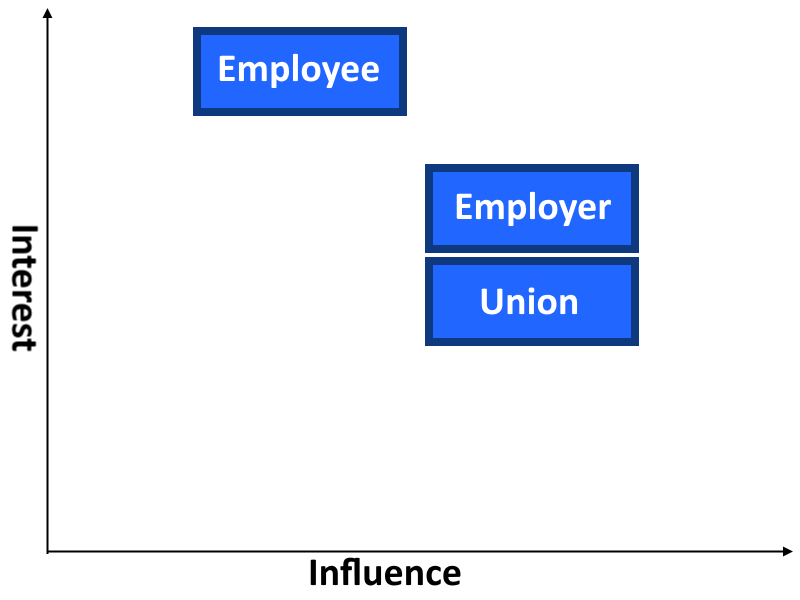
\includegraphics[width=100mm]{media/Interested Parties.png}
    \caption{Visualization of the interested parties, relative to interest and influence}
    \label{fig:Interested parties graph}
\end{figure}

As visualized in figure \ref{fig:Interested parties graph}, the employee is the party with the greatest interest since it affects their lives directly. Although, it is also the party with the least influence, since they do not have the biggest influence in demands and requirements, after all it is the union that is in control of that. We've placed the union party and the employer party at the same level of influence, but the employer has a bit more interest than the union. They have the same influence since they are the two parties responsible for making an agreement on how to treat the employees, but the employer has a greater interest since they are affected more directly than the union. The employer is responsible for following the agreement, and can face big consequences if the agreement is broken. Beyond that, the employer is making money off of the employees, hence a greater interest since it affects their income and therefore their lives.

\section{Existing solutions}
In this section we will be looking at preexisting solutions to see how these solutions approach the problem. By doing this we will be able to find out which things we should include, which things we should try to improve upon, and what we should avoid doing.

We will in addition to the above be examining the solution currently in use at \siemens, for the sake having a reference to compare other existing solutions as well as the solution we will be developing later on in the project.

\subsection{Current solution at \siemens}
This is the method that is currently being used in our case study. Once a year, one person, who is responsible for time planning, sits down and makes the plan for the entire next year. Making the schedule takes about one day for an experienced worker, however the plan has to be accepted by the employers and the employees for it to take effect. If it does not get accepted, that means there needs to be made a new one, with a new system, so that it differs from the not-accepted previous schedule. A program would also be useful later, when a new worker might have to make schedules, after the old worker resigned, saving even more time

%Not only does this take an excessive amount of time, which could be saved if a program was to be made instead, but it is also some of the most mundane and repetitive work there is to do. 


\subsubsection{Microsoft Excel}
Currently, Microsoft Excel is the preferred method of time-planning for \siemens, this is because of its cell and row system, which makes it easy to understand at a quick glance, but it also uses a mathematical function system, which allows calculations which can be dynamic, meaning that if you change a number in one cell, linked cells can get changed as well.

Currently the time-planner is given a schedule, following the example in table \ref{tab:exampleSchedule}, which can be seen on page \pageref{tab:exampleSchedule}. But this schedule does not account for vacation, public holidays like Easter or the amount of hours per year the teams should work. Therefore these things need to be fixed, and time slots in the schedule need to be either removed, or added, to make sure production keeps happening, and that the union agreement is upheld and the workers are happy.

\subsection{TimePlan}
TimePlan is a piece of software developed by TimePlan Software A / S. The program can be used to create work schedules either manually or automatically. In addition to this the program can also warn the user in case the work schedule is in breach of either a union agreement or other relevant laws. The system also supports tracking of overtime, absence, vacation, holidays, and more. All these various pieces of information can then be exported to be passed to other separate systems for payroll processing. \parencite{TimePlan}

\subsection{Planday}
Planday is a piece of scheduling-software developed by the company of the same name. It is used by several major companies such as Best Western, Just Eat, and Wolford. Planday helps the person(s) in charge of creating the schedule by making factors such as vacation, availability, etc. more accessible and easier to organize. It is therefore not completely automated, since the organizer must still finish the schedule by himself/herself, but Planday's tools makes this process much easier and less time consuming. Planday also makes it possible for employees to make suggestions themselves. \parencite{planday}

\subsection{Smartplan}
Smartplan is a system that aids in planning and managing a work schedule. Like Planday, Smartplan is not automated so the end user will still be doing some of the work. According to their website, it does offer various functions that attempt to make the process easier. It allows creating schedule templates that can be copied and filled in so that the general framework for the schedule can be reused.
It can track the amount of hours and other statistics that can used to setup rules in the system that it will then enforce for the schedule. It allows the employees to make request in addition to allowing them to take up open shifts in the schedule. While the system is not fully automatic it is capable of making suggestions based on the given rules and employee requests.

Much like TimePlan, Smartplan also offers functionality for exporting payroll information and is capable of tracking vacation, absence, and leave. Smartplan also offers functionality that lies slightly outside the scope of work schedule planning such as a clock-in (timetracking) system and general purpose internal communications system. \parencite{smartplan}

\subsection{Other options}
Other software or websites for scheduling are mainly used for smaller groups, retail and restaurants. Where the product is service, this means the scheduling is largely based on when a given customer base is normally there e.g 18:00-20:00 at a restaurant where more waiters and such are needed. The software is made to accommodate this and schedules are made within given groups for example; we need six waiters between 16:00 and 22:00 Monday till Thursday and 10 waiters from Friday till Sunday, the software would then use this information to make a schedule for everyone and give them the amount of hours specified, these kind of schedules are typically made for a couple of weeks at a time and switched between people to keep the scheduling "fair".

% summary and conclusion (what do the solutions have in common, how do they differ, what have we learned from it)
\subsection{Summary}
A general trend that seems to appear between many of the preexisting solutions is that there are a lot of interconnecting systems besides just work schedule planning. The makes sense since something like a payroll is intrinsically tied to the amount of regular and overtime hours an employee has worked along with knowing whether the employee has worked during a time slot, where they are entitled to additional pay.
\section{Data Description} \label{section:datadesc}
The data we will be working with in this project will come directly from \siemens. Although this data is not public, we have been allowed to use it in this project, and additionally put the full spreadsheet in appendix \ref{appendix:local-agreements}.

What we have received is a spreadsheet from the Human Resources (HR) department on the local \siemens facility in Aalborg. This department produces a schedule that needs to be looked over by a worker, to ensure that the schedule follows all union agreements. The spreadsheet from HR comes noted with what holidays and SH-days there are, but shifts are not accommodated in this spreadsheet. It is therefore the responsibility of the worker fixing the schedule to:

\begin{itemize}
    \item Accommodate holidays
    \item Accommodate SH-days
    \item Plan 3 weeks vacation in the summertime
    \item Plan 1 week vacation around Christmas
    \item Finally, make sure that all teams have their planned hours according to the union agreement
\end{itemize}

\begin{figure}[ht!]
    \centering
    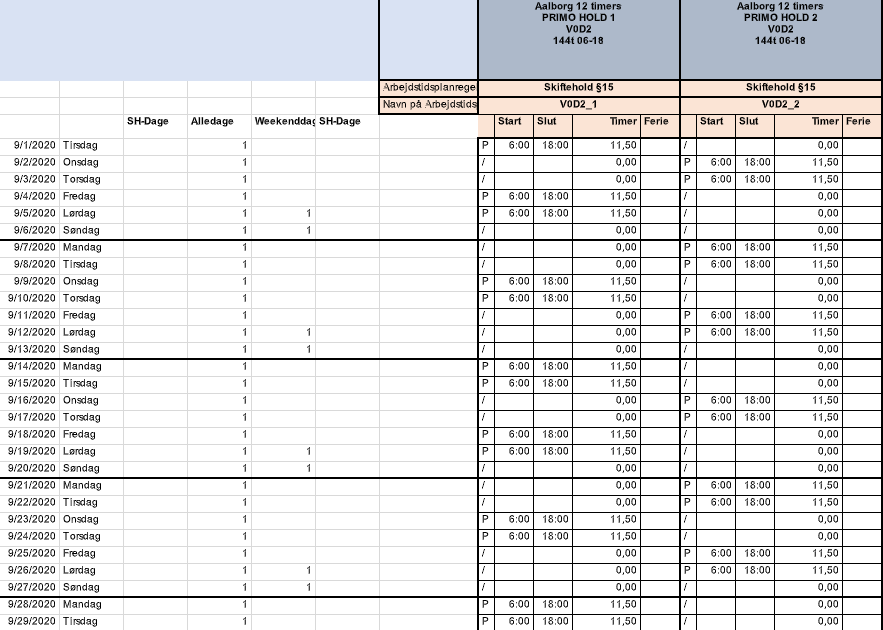
\includegraphics[width=\textwidth]{media/Schedule WO fix.png}
    \caption{Schedule that the planner receives, and then has to turn into a real schedule.}
    %first draft of the schedule proposed by Human Resources
    \label{fig:Schedule no fix}
\end{figure}

The schedule that comes in has the same structure as the example given in table \ref{tab:exampleSchedule} which can be found on page \pageref{tab:exampleSchedule}. The schedule has four teams, two day shift, and two night shift teams. We will primarily be focusing on the day shift teams, but if there is enough time we will try to make the program able to also fix the scheduling for the night shift teams. The day shift team will from here on out be called \primo team 1 and 2.


\primo team 1, as an example, works two days 6am-6pm, and then they have two days off. In those two days off, \primo team 2 works instead, which allows for production everyday, with time off. This however does not work out with a seven day work week, which is why these teams work six day work weeks. This explains why the schedule is called a 144h as well.


In figure \ref{fig:Schedule no fix} you can see the schedule given to the worker fixing it. This spreadsheet goes down 365 cells, for all the days until the next schedule needs to be. In figure \ref{fig:Schedule formated} you can see the fully formatted schedule, which is how we want the schedule to end up. This is because this is how the workers have come to expect their schedule.

\begin{figure}[ht!]
    \centering
    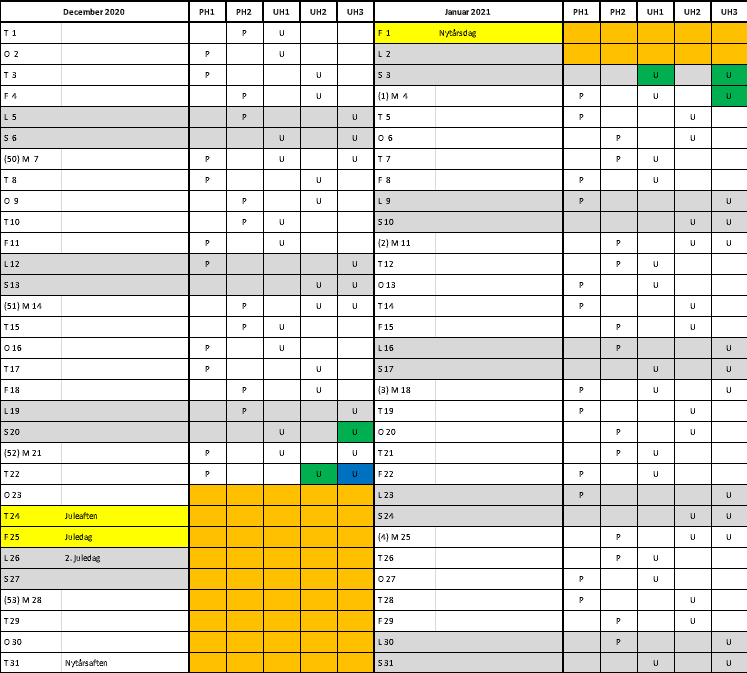
\includegraphics[width=\textwidth]{media/Schedule formated.png}
    \caption{Schedule after the planner has formatted it.}
    %Template for the final version of the schedule
    \label{fig:Schedule formated}
\end{figure}



\iffalse

The data is a spreadsheet that comes in directly from the Human Resources department. The spreadsheet has the same layout as seen in table \ref{tab:exampleSchedule} which can be found on page \pageref{tab:exampleSchedule}. Additionally the spreadsheet comes with small inputs directly from the local agreement, which helps the worker fixing the schedule, so they easily can reference different numbers like maximum hours per week.

At the end of the project, we want to create a C program that accepts the spreadsheet as a 'Semicolon-separated values'-file (\verb|.csv|), and output one as well. The program would analyse the data, see what worker shifts it should add or remove, and finally it should print it out as a schedule that is easy for the workers working the shifts to understand.

\fi
 %temporary tex
\section{Problem Definition}
Based on our analysis, we can conclude that different parties have different interests in our project. They all want a fair, efficient, and predictable program, that reliably creates a work schedule. We have chosen to focus on the work scheduling at \siemens for the shift teams, where we will make a usable work schedule (Figure \ref{fig:Schedule formated}) from a proposed schedule (Figure \ref{fig:Schedule no fix}). Based on this we have come to the following problem definition:

\begin{quote}
    How can we create a program that automates the process of taking a proposed timetable  from \siemens and making it into a proper work schedule, with the goal of minimizing work hours spent making it?
\end{quote}

We want the program to reliably create a work schedule, that follows the requirements of the union and local agreements. This means it shall be able to calculate the different average working hours, and accumulated work hours. It should also be able to place the shifts on valid days, such that Sundays are avoided. Out from the information of the accumulated working hours the program should be able to determine how many shifts needs to be added or removed and give potential shifts to remove or add to make the production still run smoothly. The program should also create the work schedule fast and reliably, making sure that as little time as possible is spent on creating the actual work schedule. Furthermore, it should be able to divide work on holidays equally between the teams, as to make sure that no one team is working more on undesirable shifts than the other teams.

% Solution/development
\chapter{Solution development}
In this chapter we will be documenting the development process of our solution.
This will include requirements of the program, and specifications of how the input and outputs will be given and how they are expected to be formatted.


\section{Requirements}
In this section we will be outlining the requirements of our program. We will be separating the various requirements by priority. Some of our requirements are significantly more important than others, and the ones of lower priority may not end up being implemented if the available time proves to be insufficient.

Our programs requirements are listed as following (each of the requirements is marked with a number representing its priority):
\begin{itemize}
    \reqItem[1]{Input/Output}{Since we need to import the data from an Excel document, we need to figure how exactly to do this. Since, the Excel format is quite complicated we want to take a simpler approach. As such we want to use a \textit{semicolon separated value} format, which Excel has native export and import support for.}
    
    \item[] \textbf{Union and local agreements:} The program needs be able to create a schedule that upholds the union and local agreements, regarding working hours and shift placement.
    
    \item[] \textbf{SH-days:} The program needs to take holidays (SH-days) into account.
    
    \item[] \textbf{Work hours:} The program should ensure that each of the teams do not exceed the expected hours or have an insufficient amount of hours, and remove or add shifts accordingly. Here public holidays and Saturdays should be prioritized over other days, if a shift is able to be removed.
    
    The program must accumulate the work hours and include them with the resulting schedule.
    
    \reqItem{Days in a year}{Since the year does not start at the same weekday each year we have a different number of weekends each year. Our program should be able to allocate memory according to the number of days, weeks and weekends, in that specific year.}
    
    \item[2] \textbf{Leap years:} The program should be able to change the schedule accordingly if the year is a leap year.
    
    \item[\textbf{3}] \textbf{Schedule criteria:} In the case of a proposed schedule being rejected we would need to generate a new one that can take the needed adjustments into account. In this case we would have to generate a new schedule, and to do that we need to define a format and method by which the end user can supply adjustments to the schedule.
    
    \item[\textbf{4}] \textbf{Option flags:} There can be the option to flag your output file, for example give it a specific name instead of the programmed standard name.
    
    \item[] \textbf{GUI:} The program should have a graphical user interface.
    
    \reqItem[5]{Excel file}{The program should output a more user-friendly file-format like a \texttt{.xml} file instead of a \texttt{.csv} file. It would be more user friendly, as the schedule would be able to add the different colours if needed, as well as generating a better looking layout.}
\end{itemize}



\section{Program Description}
In this section we will be going over how the program as a whole will function, using flowcharts to illustrate the flow of the program. In the below figure (\ref{fig:Main_Flowchart}) the overall flow of the program can be seen. As we mentioned in the requirements section the program will be accepting a \verb|.csv| file. This input file first has to be read and parsed in order to convert the file into a data structure that we can use within our program. Once the input file has been processed we need to determine if any changes are necessary. This is done by comparing the expected work time (from the input file) with the work time that has been scheduled so far.

%fix later
\if1
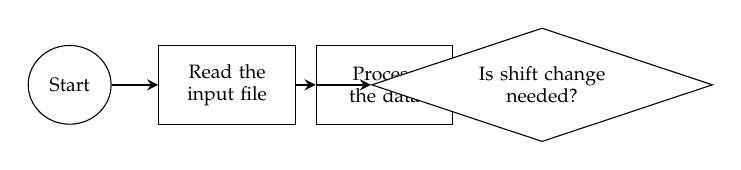
\begin{tikzpicture}[node distance=2cm,font=\scriptsize]
    \node (start) [startstop] {Start};
    \node (read) [process, right of=start, text width=1.5cm] {Read the input file};
    \node (proc) [process, right of=read, text width=1.5cm] {Process the data};
    \node (need) [decision, right of=proc, text width=2cm, aspect=3] {Is shift change needed?};
    \draw [arrow] (start) -- (read);
    \draw [arrow] (read) -- (proc);
    \draw [arrow] (proc) -- (need);
\end{tikzpicture}
\fi

\begin{figure}[ht!]
    \centering
    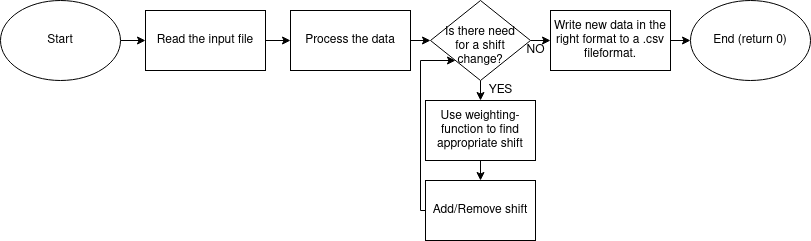
\includegraphics[width=\textwidth]{media/Flowcharts/General flowchart.png}
    \caption{Flowchart of the program flow.}
    \label{fig:Main_Flowchart}
\end{figure}

If there is either too much or too little work time scheduled the program will remove or add scheduled time, respectively. In order to determine where to add or remove a time slot a weighting function will be used. Once a time slot has been removed or added the program will once again check the total time and compare it to the expected amount. If they match, the program will proceed. Otherwise, the aforementioned process will repeat. Once this process has finished the resulting schedule will be formatted and written to a file.

As mentioned the weighting function will be used to determine which time slot should be added or removed. It does this by giving each time slot a score, here the highest score will be the time slot which will be removed and the lowest score will be added. A flowchart of this function can be seen on Figure \ref{fig:weighting_flow}.

\clearpage
\begin{figure}[ht!]
    \centering
    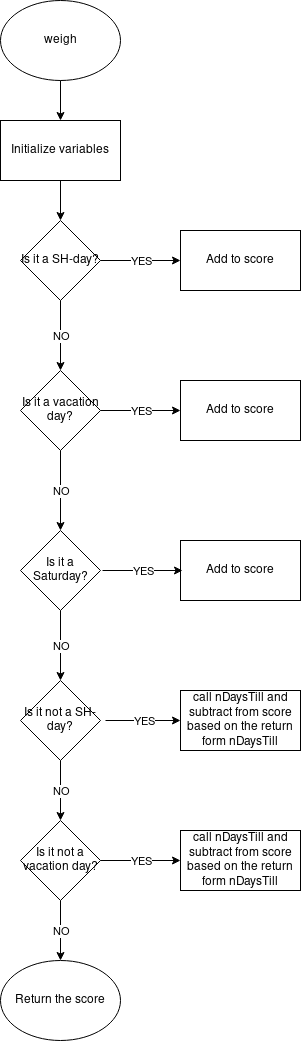
\includegraphics[width=0.8\textwidth]{media/Flowcharts/weight_flow.png}
    \caption{Weighting function flowchart.}
    \label{fig:weighting_flow}
\end{figure}

The most important part of the function is the four if-statements and the code being run if these turn out to be true or false in the case of the first three. The first if statement checks to see if the exceed the amount of work hours we can have in a week. If, we do then the time slot needs to have a really high score because we can not have to many hours in a week. Does it turn out to e false we add to the scored based on the amount of hours in the week. In the next three statements we check whether or not it is a specific type of day. If it is we add to the score. This means that time slots on these days will get a better score. The middle two if statements also have an else condition. If it is not an SH-day we calculate the number of days too the closest SH-day. We then multiply the number of days with a constant and subtract that from the score. The same process is done for vacation days. 

To calculate the aforementioned number of days we use the nDaysTill function. A flowchart for that con be seen on Figure \ref{fig:flow_nDaysTill}.

\clearpage
\begin{figure}[ht!]
    \centering
    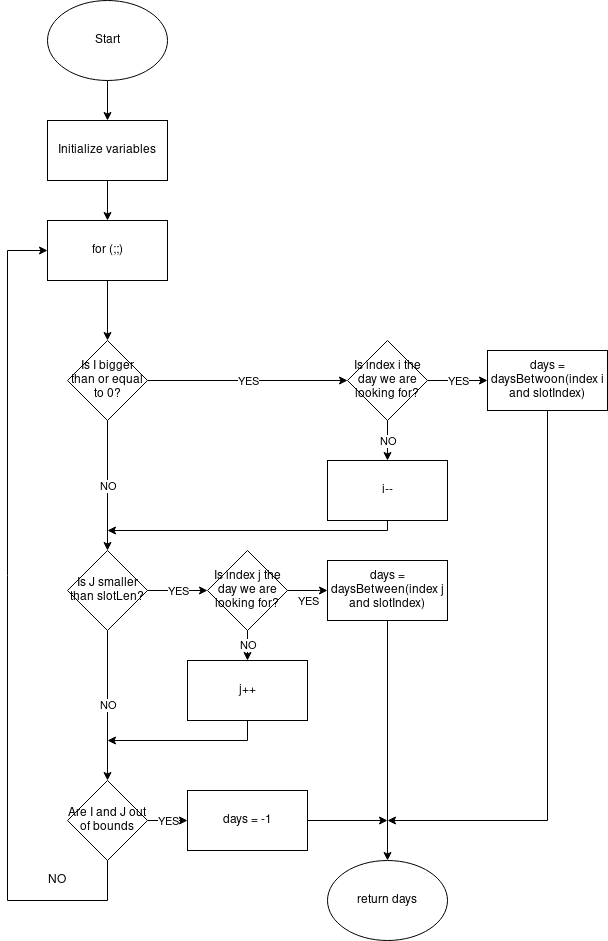
\includegraphics[width=\textwidth]{media/Flowcharts/nDaysTill_flow.png}
    \caption{Flowchart for the nDaysTill function.}
    \label{fig:flow_nDaysTill}
\end{figure}

This function starts off by making two index variables (i and j) based on an index it gets as a parameter. The first is going to go backwards in a time slot array and the other is going to go forwards in the same array. We then go into an infinite loop. In the loop there are three if statements, the first checks whether i is out of the array bounds, the second does the same but for j and the last checks both the variables. If the first if statement is true we then check to see if the time slot at index i is on the day that we are looking for, if it is we calculate the number of days between the time slot at the index given as a parameter and the time slot at index i. We then break out of the loop and return the number of days. If it turns out that it is not the day we are looking for we subtract one from i and go back to the for loop right after the first if statement. The second if statement has the same process as the first except this time we check j. Lastly we check to see if both index variables are out of the array bounds, and if they are we break out of the loop and return -1.p
\section{Specification and design}
In this section we will be covering the specification and design of our program. The purpose of the specification is to provide a clear cut definition for what the program is supposed to do and how it is to be approached.

\subsection{Inputs and outputs}
In this section we will be specifying the inputs and outputs for our program.

\subsubsection{Input}
As we mentioned in the requirements related to Input/Output, the native Excel file format \verb|.xlsx| is fairly complicated. We have decided that we will be using \verb|.csv| files instead. Excel has built-in functions for exporting and importing \verb|.csv| files, so this should still be fairly easy for the end user of the program to make use of.

The program should take a path to the input file as the first argument when invoking the program from the command line. This will in addition allow the program to be executed by drag and dropping a file onto the executable on Windows (and potentially other operating systems).

The output file should reuse the name of the input file with the word \textit{out} in-fixed between the end of the name and the file extension. Optionally the output file can be specified by providing the \verb|-o| flag followed by a file path when executing the program.

The input file we have been given as an example consists of seven columns and 13 rows of information. This is the information that would be available for a person manually fixing the schedule. Information like how many hours a team should have per day or week, or how many public holidays there are in a specific year. This means that the program should start from the eighth column and 14th row, and look at the rest of the sheet from that. The data that has come and needs to be processed, is in the same format as Table \ref{tab:exampleSchedule} which can be found on page \pageref{tab:exampleSchedule}. Additional information can be found in Section \ref{section:datadesc}.

\subsubsection{Output}
For the output file we are going to recreate the style that is used on \ref{fig:Schedule formated}. This can not be done perfectly since the end result has some color coding, and we can not do that information in a .csv file, we can only specify what information goes into each cell. Therefore we have to get a little creative. Each color in the Excel file is going to get replaced by a character or symbol. Luckily there is not much text in the schedule so if we pick the right symbols it should be easy to find and replace the symbols with color coding if the user really want to. The new coding is as follows:

\begin{itemize}
    \reqItem{Removed}{Green $\rightarrow$ RM}
    \reqItem{Added}{Blue $\rightarrow$ AD}
    \reqItem{SH-day}{Yellow $\rightarrow$ SH}
    \reqItem{Vacation}{Orange $\rightarrow$ VC}
\end{itemize}

The only one you can find in the schedule right now is RM, which shows up once. It should therefore be very easy to replace these if the user deems it necessary. 

Now as for how we are going to write it to our output file. In our heads it might make more sense to calculate one month at a time, starting at the first one and then continuing chronologically. However, it makes much more sense computationally to do it row by row. This is because each line in the .csv file is a row in our schedule. We can make a single line at a time and write it to the .csv file, and then forget about it. However, working month to month is still possible, as the output will be a file the program have full access to, meaning it can change every single line at any time if necessary.

One thing that we should keep track of though is all the special days. This being the SH-days, holidays, removed days and added days. We should definitely add this to the bottom of the schedule, as seen in the template. We need to show the information of these days as the user will have to mark these days with colors, and to check if any significant changes has been made.

The following is an example of how the final work schedule should look:

\begin{figure}[ht!]
    \centering
    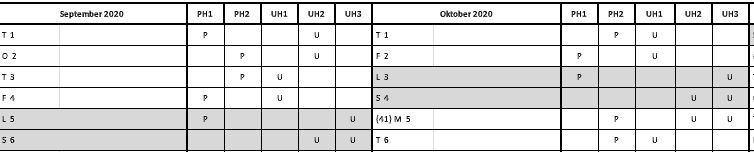
\includegraphics[width=\textwidth]{media/p1 schedule.JPG}
    \caption{The final work schedule example.}
    \label{fig:Output_example}
\end{figure}
 In the following chapter we will show how to read a csv. file, which is also how we need to make the program write out the final file. Excel will then be able to show the final schedule by interpreting the csv. file.

\subsubsection{Analysis of the input format}
\label{sec:input-analysis}
In this section we will be doing an in depth analysis of the input document format. The full document can be found through appendix \ref{appendix:local-agreements}.

The \verb|.csv| file format consist of multiple strings, separated by semicolons. Each string represents the value in the current column and each semi-colon represents the transition from one column to the next. Rows are separated by line breaks. Each row has the same total amount of semi-colons, this means that when a column is empty multiple semicolons may appear back to back.

A single day in the input timetable will be represented with the following line of data, in a \verb|.csv| file (note that the line is broken for the sake of readability, the listing represents one entire row):

\begin{lstlisting}[caption={Example row.}]
    9/1/2020;Tirsdag;;1;;;;P;6:00;18:00;11,50;;/
    ;;;0,00;;/;;;0,00;;U;18:00;6:00;11,50;
\end{lstlisting}

The first column contains the date, in this case \textit{"9/1/2020"}. The date is followed by the weekday in the proceeding column. In the next (third) column we can find the name of the SH-day, since the day used for this example is not an SH-day the column is left empty. For the next three columns the value is either omitted or \textit{"1"}. These columns are used to identify what kind of day it is, the first is always set and simply means that it is a day. The second column is used for identifying weekend days and the third for SH-days. The next column is always empty.

Then we reach a "P". This means that \primo team 1 has a shift this day. Then the hours come, from six to 18, and how many hours that is in paid work. Then two semicolons later, we meet a "/". This represents that the \primo team 2 does not have a shift this day. and therefore, there are no hours entered in the next two columns. Then the hours of the day is in the next column, and because there are no work hours, "0,00" is entered. The same is the case for the \ultimo team 1, that does not have a shift, and there therefore is a "/". The \ultimo team 2 however does have a shift, because there is a U, and then their hours. Then the next row of the Excel file will be on the next line. From now on we will not be showing the semicolon separated string, but instead the tables, as it is explained above how a table will be written as a semicolon separated file.

There is one more important information in the Excel file that we need our program to be able to read. That is the table at the top, that shows how many days, holidays, workdays and hours the different teams have with the current schedule.
 
\begin{figure}[ht!]
    \centering
    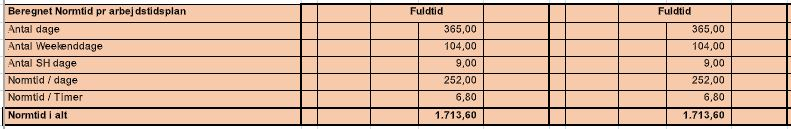
\includegraphics[width=\textwidth]{media/Table P2.JPG}
    \caption{Table of general information.}
    \label{fig:Table_information}
\end{figure}

We need to get the program to store the accumulated hours, as to know how many hours the teams should optimally have this year. The other information does not seem as important, as we will most likely gain the same values, when we store all the different days.


\subsubsection{In code representation of the input}
In this section we will be documenting some of the considerations we have made in regards to the in-code representation of the input format.

As we went over in the section on input analysis (see \ref{sec:input-analysis}) the input source is a text file containing multiple rows each containing a series of information about the given time slot that the row represents. Since we have many rows that all follow the same format the obvious solution is to make use of an array to store each row. It is however less obvious how to store the information contained within each of these rows.

The overall plan is to organize the contents of a row into a data structure. With that said we probably won't be using all of the fields, since some of the information is slightly redundant. In addition some of the representations used within the source data, would likely prove inconvenient to work with and as such we will be changing those to be more convenient.

The first field is the date of the given time slot. The original representation uses the following format \verb|month/day/year|. This should have its own data structure, with separate fields for month, day, and year.

The second field stores the name of the weekday. Instead of storing this as a string directly, we should convert it to a numeric representation with zero representing Monday and seven representing Sunday. To represent this in code we will be using an enumeration type.

The third field is the name of the SH-day. This field is only needed for outputting as text in the final schedule, as such it should simply be stored as a string.

As for the next three fields, they can be omitted since the other fields carry more than enough information to infer the value of these. For reference these fields state whether the time slot is on a day, a weekend day, or a SH-day.

For the remaining 20 fields there is a repeating pattern across four sections of five fields. The first of these five fields determines which team is working. The next two fields contain the start and end times for shift respectively, the fourth contains how many work hours the shift is equivalent to. The last field is unused and will be omitted.

For the start and end times, we will be using a simple data structure with a field for hours and minutes. For the field containing the work hour count we will simply be using an integer for storing the work time in minutes (since minutes is the smallest unit used in this case). 
The time slots will be divided up into arrays based on the team it is associated with.

\begin{lstlisting}[caption={Example data structure.},language=C]
    typedef struct {
        Date date;
        Weekday day;
        const char* shName;
        Time startTime;
        Time endTime;
        int workHours;
    } Timeslot;
\end{lstlisting}

\subsection{Creating the work schedule}
In this section we will specify how our program will create the work schedule.

The program checks how many hours the current plan gives each team, and then calculates the difference between the planned hours and the hours agreed upon according to the union agreement. If the planned hours exceed the agreed upon hours by more than than one shift, meaning 11.5 hours, the program should find the most optimal shift to remove. This means that the program should check if they are working on a SH-day, and remove that shift. If that is not possible it should then instead find a Saturday they work and remove that one. It should prioritize removing days that are particularly annoying to work on, such as days right before or after SH-days, or in periods of time where they have not had many days off. However the program should also keep in mind, that we are going for constant production at \siemens, so we should not have a day with no shifts. We can allow a small team like Ultimo team 3 to close production alone, if it is more optimal to remove other shifts. The employees would most likely prefer this method over just choosing random days, since this method is more convenient.

On the other hand, if they are below the amount of hours needed, an extra shift should be added. The program needs to find a day that the team are not working and add a shift to that day. This day should also be carefully chosen. If a normal day is possible, it should be added there, but if that is not possible, then they should add it to a Saturday as far away from holidays as possible. Only if no such day exits should it place the shift on a SH-day.


\section{Source code structure}
In the following section we will describe how the structure of our program will be. The program will be written in the language C, which means we can split our programs directory into separate C source files (\verb|.c|), and link them together using header files (\verb|.h|). In each of the following subsections, we will describe each file, both C source files, and header files.

\subsection{main.c}
The \verb|main.c| file will acts as our main file, where we use the functions and data types from the other files to solve our problem and make a work schedule in the right format. This file is the only one to include header files for all of the other files in our program, since it is the main file and needs the attributions from all of the other files.

\subsection{types.c/.h}
The \verb|types.c| will be containing the structs and data types that we will be using in our program. This file will be used as a header in most, if not all, other files.

\subsection{input.c/.h}
The \verb|input.c| file will contain the code required to scan the initial work schedule (Figure \ref{fig:Schedule no fix}), and insert it into the data types made in \verb|types.c|, which means it needs to include a header file, pointing towards \verb|types.c|.

\subsection{outputwriter.c/.h}
The \verb|outputwriter.c| file will contain the code that writes all of our data, processed in \verb|main.c|, out to a "Comma Separated Varia
ble" file, in the right format, as seen in Figure \ref{fig:Schedule formated}.

\subsection{gen.c/.h}
The \verb|gen.c| file will be used to generate most, if not all of the schedule. This file will also be dependant on the \verb|types.c| as a header file.

\subsection{Illustration}
All of the dependencies can be explained in an illustration


\section{Implementation}
In this section we will be going over the implementation process for our program. We will be documenting some of the choices that have been made throughout the development process.

\subsection{Time slot storage}
One of the things we needed to figure out how to handle was storage of the time slots that we load from the input file. Unfortunately we do not always know how many time slots exist for each team as such we can not simply allocate a predetermined amount of memory.

To solve this we decided to implement a dynamically allocated expansible array. For this array we needed a few different functions. Firstly we needed to create and initialize a new array, this includes allocating storage for a given amount of elements. Secondly we want to be able to easily add an element to the end of the array. This would also include expanding the array when there is insufficient space available, which leads to the third function, reallocation and copying of elements. Lastly we need to be able to free the memory.

In order to make this possible we want to track the amount of elements currently in the array, along with amount of elements that can be stored in the array. We have implemented this as a data structure as seen in listing \ref{lst:struct-tslist}.
\begin{lstlisting}[caption={Definition of the list structure},label={lst:struct-tslist},language=C]
    typedef struct {
        /* The total amount of elements that
           can be stored */
        size_t capacity;
        
        /* The amount of elements currently
           stored in the array */
        size_t length;
        
        /* A pointer to the memory where the
           elements are stored */
        Timeslot* storage;
    } TsList;
\end{lstlisting}
With this in mind we have declared the four aforementioned functions as seen in listing \ref{lst:funcs-tslist}. All functions, except \verb|tsListNew|, takes a reference to an existing \verb|TsList|. Both \verb|tsListNew| and \verb|tsListRealloc| takes a value of type \verb|size_t|, which is used for specifying the capacity of the list.
\begin{lstlisting}[caption={Declarations of TsList functions.},label={lst:funcs-tslist},language=C]
    /* Reallocates and copies the list storage. */
    void tsListRealloc(TsList*, size_t);

    /* Creates and initialises the list. */
    TsList tsListNew(size_t);

    /* Pushes an element to the end of the list. */
    size_t tsListPush(TsList*, Timeslot);

    /* Frees the memory used by the list. */
    void tsListFree(TsList*);

\end{lstlisting}

\subsection{Reading data into the time slots}
We will have an array of time slot lists, where each time slot list represents a team at \siemens. We will create a new struct that holds a time slot list and the anticipated hours of each team. The first values we read into this struct will be the anticipated hours of each team, as they are the first to appear in the .csv file. We will check that we do not suddenly reach the end of the file, as that would mean the wrong input-file has been given to the function. If that is not the case, we go to the next part of the input:

We skip ahead by 17 lines until we get to the actual dates and shifts. Here we read the date into a temporary time slot, with a function that separates the string in the form "dd-mm-yyyy" and into three unsigned integer values. Then we read the name of the weekday, and if it is a holiday. If, it is a holiday then the holidays name also is loaded into the temporary time slot. We then check for each team if they have a shift that day, by checking if any hours are present. We then load the start and end time of the shift into the temporary time slot, and the amount of work hours converted to minutes are also loaded into the time slot. The time slot is then pushed to the appropriate teams time slot list. Lastly we overwrite the start and end time and work hours with the next teams shift, and then push that time slot to the next teams time slot list and so forth for each team. When we reach the end of the line, we go to the next day, and reset the temporary time slot. 

\subsection{Keeping track of allocated strings}
While parsing the input file we have to allocate memory to store the strings in (in particular the names of SH-days). Whenever we allocate memory we of course have to free once we are done with it. One way to accomplish this would be to iterate through all the time slots and freeing each string as we encounter them. This has the downside that we iterate through a large amount of time slots that do not have any strings associated with them. To minimize excess iterations we can store a reference to each string in a separate table. For this we have considered using either an  array or linked list to keep track of the references. The benefit of an array is that a new reference can be added in $O(1)$ time vs $O(n)$ for a linked list. But the downside is that we will have to either make assumptions about the amount of strings that needs to be stored or have to resize the array as we go, which can be rather expensive since it can result in copying the entire array. We assume that there is a relatively small amount of SH-day names and with this in mind we think that the ease of extension outweighs the cost of insertion and thus we have chosen to use a linked list.

\subsection{Assigning a weight to each time slot}
The weigh function is a function that takes four inputs. An array of time slot structs, the length of the array, an array of user defined constants and index in the array. The function will then return an integer value for the time slot needed at that index in the array. This integer is a score for that time slot, which represents how good it would be to give the workers time off in that time slot. This way we can remove the highest scoring day if the workers are working too much or add in the lowest scoring day if they are working too little. 

The function itself is pretty simple. We have some specific days that we value higher than others, those being SH-days, vacation days and Saturdays, if the time slot is in one of those days we up the score by a certain amount. We also want to give a higher score to time slots closer to a SH-day and vacation day. We also to spread the free days out a little bit so the work hours in the week is also taken into account. The code for the function can be seen on Listing \ref{lst:weigh}.

\begin{lstlisting}[caption={Weigh function.}, label={lst:weigh}, language=c]
/*given an array of timeslots the length of the array and and an index, return the score of the timeslot of that index*/
int weigh(Timeslot slots[], int slotsLen,
          char* modifiers[5], 
          int workHours, int slotIndex) {
    /*the constant scores and multipliers should optionally be changed by flags*/
    int score = 0, 
        scanned_modifiers[] = {500, 50, 200, 2, 1};

    if (workHours > 4 * 690) {
        score = INT_MAX / 2;
    } else {
        score += 5 * workHours;
    }

    /*if we have gotten any flags specifying values for the modifiers scan them and assign the value*/
    for (int i = 0; i < 5; i++) {
        if (modifiers[i] != NULL) {
            sscanf(modifiers[i], "%d", 
                   &scanned_modifiers[i]); 
        }
    }

    /*if it is an shDay add to the score if it is not find the closest sh day and subtract from the score*/
    if ((slots + slotIndex)->editState == ShDay) {
        score += scanned_modifiers[0];
    } else {
        score -= scanned_modifiers[4] * 
                 nDaysTill(slots, slotsLen, 
                           slotIndex, ShDay);
    }

    /*if it is an vacation add to the score if it is not find the closest vacation and subtract from the score*/
    if ((slots + slotIndex)->editState == Vacation) {
        score += scanned_modifiers[1];
    } else {
        score -= scanned_modifiers[3] *
                 nDaysTill(slots, slotsLen,
                           slotIndex, Vacation);
    }

    /*if it is a saturday add to the score*/
    if ((slots + slotIndex)->weekday == Saturday)
        score += scanned_modifiers[2];

    return score;
}
\end{lstlisting}

The function takes 5 parameters, an array of time slot, the length of this array, an array of user defined weights, the number of workhours in the the current week and lastly the index for the time slot we want to give a score. It starts of by initializing the score as an integer and an array of modifiers with default values for the previously mentioned constants. The function then checks to see if we have too many work hours in the current week and adds too the score accordingly. Then we read the user defined modifiers if there are any (more on this later). After reading the modifiers we check for all the specific days and add to the score if it is any or multiple of them. If the time slot is not on an SH-day day we subtract from the score based on the number of days until the closest one, this is also done if it is not on a vacation day. This is done using the nDaysTill function. Once, we have run through all of our scoring criteria we can return the score.

\subsubsection{Finding the next day of a specific type}
The nDaysTill function takes four parameters. Three of which are the same as the weigh function and then an integer which will represent a specific day from our editState enumerator. The function will then return the number of days from the day of the time slot at the index parameter (slotIndex) to the closest day which has the given editState. The code can be seen below on Listing \ref{lst:nDaysTill}.

\begin{lstlisting}[caption={nDaysTill function.}, label={lst:nDaysTill}, language=c]
/*given the on array of timeslots the length of the array and an index return the number of days to a sh-day*/
int nDaysTill(Timeslot slots[], int slotLen, int slotIndex, int editStateDay) {
    /* days until the next sh-day
     * index variable for going backwards 
     * index vairable for going forwards */
    int days = 0, 
        i = slotIndex - 1,
        j = slotIndex + 1;


    /*if the day itself is not an sh-day we want to find the nearest day which is*/
    for (;;) {
        /*if i is larger than or equal to zero then if the day at index i as sh-day set day equals i and break, otherwise go to the previous day*/
        if (i >= 0) {
            if ((slots + i)->editState == editStateDay) {
                days=daysBetweenDates((slots + i)->date,
                                      (slots +
                                       slotIndex)->date);
                break;
            } else {
                i--;
            }
            
        }

        /*the same as before but now we go forwards*/
        if (j < slotLen) {
            if ((slots + j)->editState == editStateDay) {
                days=daysBetweenDates((slots +  
                                       slotIndex)->date,
                                      (slots + j)->date);
                break;
            } else {
                j++;
            }
        }
        
        /*this should really never happen*/
        if (i < 0 && j >= slotLen) {
            days = -1;
            break; 
        } 
    } 

    return days;
}
\end{lstlisting}

We start the function by initializing three variables. All three being integers, the first is the number of days, the second being the index (i) before our parameter slotIndex and the last being the index (j) after the aforementioned slotIndex. 

In the function there is an infinite for loop which contains three if statements. In the first we check whether i is bigger than or equal to zero. If that is the case we check to see if the time slot is on the day that we are looking for. If it is, we find the number of days between the time slot at index slotIndex and the time slot at index i, then we break out of the loop. If it is not the day we are looking for we subtract one from i. This means we are going further back in the array of time slots. In the second if statement we do pretty much the same except we are now going forward in the array and using the variable j instead, meaning we check time slots at later dates instead of earlier dates. In the last if statement we check to see if both index variables are out of the array bounds. If they are it means that there are not any time slots on the specific day that we are looking for, and we then break out of the loop.

In the end we return the number of days or minus one if we do not find the day we were looking for.

\subsubsection{Finding the number of days between two dates}
The daysBetweenDates function takes two date structs and returns the number of days between them. The function also assumes that the first parameter is a date before the second parameter. The function has a single variable, that being the number of days. We run a while loop until the days, months and years are the same for both of our parameters. While we are in the loop we use the tomorrow function that takes a date struct as an input and returns the day after that. We assign the day after our first parameter to our first parameter, thus the first first parameter is now one day closer to being equal to the second parameter. We then add one to the number of days. The exit condition for the loop is when the two dates have become equal. Once, we are out of the loop we can return the number of days. The code for this can be seen on Listing \ref{lst:days_between}.

\begin{lstlisting}[caption={Days between days.}, label={lst:days_between}, language=c]
/*calculate the number of days between two dates we assume that d1 is before d2*/
int daysBetweenDates(Date d1, Date d2) {
    int days = 0;
    //while the two days are not the same go to the next day and add one to our days counter
    while((d1.day != d2.day) ||
          (d1.month != d2.month) ||
          (d1.year != d2.year)) {
        d1 = tomorrow(d1);
        days++;
    } 

    return days;
}
\end{lstlisting}

\subsubsection{Weighting user configuration}\label{WeightingConfiguration}
it can be very hard for us to narrow down some specific values to use as weights. Therefore we have made it possible for the user to use flags when using the program in a terminal. To use these you have to enter a dash followed by a the symbol then a space and lastly the number that the user wants the weight to be. The symbols and meanings are the following:

\begin{itemize}
    \item s to change the weight for the time slot being on an SH-day.
    \item f to change the weight for the time slot being on a vacation day.
    \item l to change the weight for the time slot being on a Saturday.
    \item S to change the weight when calculating the number of days to the next SH-day.
    \item F to change the weight when calculating the number of days to the next vacation day.
\end{itemize}

In the code we have a parser and we can therefore easily make some simple flags, as seen on Listing \ref{lst:user_flags}.

\begin{lstlisting}[caption={Weighting options.}, label={lst:user_flags}, language=c]
// Program option target variables.
char* input_file_path = NULL;
char* output_file_path = NULL;
char* criteria_file_path = NULL;
char* modifiers[] = {NULL, NULL, NULL, NULL, NULL};

/*
* Program option definitions.
* output file path option aling with 5 options to change default modifiers in the weigh function
* s score for being an sh-day
* l score for being a saturday
* f score for being a vacation day 
* S multiplier for when it is not an sh-day 
* F multiplier for when it is not a vacation day
*/
const Option options[] = {
        {&output_file_path, 'o'},
        {&criteria_file_path, 'c'},
        {modifiers    , 's'},
        {modifiers + 1, 'l'},
        {modifiers + 2, 'f'},
        {modifiers + 3, 'S'},
        {modifiers + 4, 'F'}
};

input_file_path = parseArgs(argc, argv, 
                            sizeof options / 
                            sizeof(Option),
                            options);
\end{lstlisting}

We can see here that we initialize all our flags as char pointers (strings) to NULL. We then make an array of options which contains sets of pointers to our flags along with a symbol. The parseArgs function is then used to parse any arguments given when the program is run.  As for the weighting function the modifiers array is then passed on until it is needed in the weigh function. We can see that here.

The weigh function is made to use integers as weights. Therefore, the user defined weights that are currently represented as strings have be scanned to integers. So in the weigh function we go through the modifiers array and check if each pointer in the array is NULL. if it is not it means that we have an input which is a number as a string. The string is then scanned for a decimal integer, and the value replaces the default value in the scanned modifiers array. The code for this can be seen on Listing \ref{lst:weigh}.

\subsection{Criteria}
The criteria as mentioned needs to be input as a file, and therefore we have to read it, we start by figuring out the size of the file so we can allocate the amount of memory needed.
\begin{lstlisting}[caption={Allocating memory in GenCriteria}, label={lst:GenCriteria_MemoryAllocation},language=C]
    int lineCounter = 0;
    /*for loop checks for EOF*/
    for (c = getc(inputFile); c != EOF; c = getc(inputFile)){
        if (c == '\n') /* Increment lineCounter if this character is a newline*/
            lineCounter = lineCounter + 1;}

    *criteriaOutput = malloc(sizeof(Criteria)*lineCounter);
/*rewind inoutFile for the rest of the function*/
    rewind(inputFile);
\end{lstlisting}
afterwards we are reading the file one line at a time until we do not get the expected amount of arguments. and then parse this into the Criteria struct.
\begin{lstlisting}[caption={Reading file in genCriteria}, label={lst:GenCriteria_FileReading},language=C]
while (fscanf(inputFile, "%s %*c %c %*c %s", buffer, &forceSchedule, team) == 3) {
        bool = 0;

        criteriaOutput[0][i].date = stringToDate(buffer);

        if (forceSchedule == 'Y') bool = 1;
        criteriaOutput[0][i].forceSchedule = bool;

        if (team[0] == 'P') {
            if (team[4] == 'O') criteriaOutput[0][i].team = PrimoOne;
            else criteriaOutput[0][i].team = PrimoTwo;
        } else {
            if (team[6] == 'O') criteriaOutput[0][i].team = UltimoOne;
            else criteriaOutput[0][i].team = UltimoTwo;
        }
        i++;

    }
    if (feof(inputFile)) {
        return i;
    } else {
        /* Errors */
        return 0;
    }
\end{lstlisting}


\subsection{Output .csv file generation}
The output file is as mentioned before a .csv file. Luckily a .csv file is just a formatted text file, using commas or semicolons as separators. This means that we can just write everything out, making sure to place the correct commas or semicolons. 

We start out with the line of code that prints out the header of the file. In listing \ref{lst:Output_header}, you can see the pseudocode representing this process, as the actual code is rather unreadable with the limited line space of this project. The header will include what period of time the schedule is made for.


\begin{lstlisting}[caption={Writing of header in pseudocode},label={lst:Output_header},language=C]
print "Fast skifteholdsplan i perioden" 
      + month_start + "-" + month_end
      + "for_timeloennede medarbejdere paa 144 timer"
\end{lstlisting}


After, this we need to print out twice. Once for each half of the schedule, since it is divided into two equally big 6 month periods, instead of a long line of 12 months in a row. Therefore, we call the function to print out the specific dates twice. First time we call it, it goes through the first six months, and checks and prints what need to be printed. After, the first time we return an integer. This integer is how many days are in the first six months. We do not always know this value, as we could have different starting dates (e.g we do not start the schedule in September, or we have a leap year), and therefore different amount of days to go forward 6 months. 

When we have the return value, we use it to call the function a second time, this time giving it our returned int, and therefore printing the months 7-12 instead of 1-6 as before.

The code:
\begin{lstlisting}[caption={Printing of dates written in pseudocode},label={lst:Date_print},language=C]
for (i = current_day; i =< last_day; i = next_day)
    day = i
    print day.weekday + day.shName;

    if(Primo_one has shift on day)
        print "P"
    if(Primo_two has shift on day)
        print "P"
    if(Ultimo_one has shift on day)
        print "U"
    if(Ultimo_two has shift on day)
        print "U"
\end{lstlisting}

%\begin{lstlisting}[caption={Printing of %dates},label={lst:Date_print},language=C]
%fprintf(file, "%c %d;%s, ", weekdayToChar(tsd->timeslotList.storage[i + %days].weekday), i + 1,
%tsd->timeslotList.storage[i + days].shName ? tsd->timeslotList.storage[i + %days].shName : " ");

%fprintf(file, "%c,", 
%        tsd[0].timeslotList.storage[i + days].workTime ? 'P' : ' ');
%fprintf(file, "%c,", 
%        tsd[1].timeslotList.storage[i + days].workTime ? 'P' : ' ');
%fprintf(file, "%c,", 
%        tsd[2].timeslotList.storage[i + days].workTime ? 'U' : ' ');
%fprintf(file, "%c,", 
%        tsd[3].timeslotList.storage[i + days].workTime ? 'U' : ' ');
%
%\end{lstlisting}
                
\section{Testing}
In this section we will be going over some of the ways we have tested the program to ensure that it works as expected. This also includes checking to ensure the program does not have any unwanted side effects such as memory leaks.

\subsection{User test}
A user test of the program was conducted during the development process. The test consisted of our \siemens contact following the instructions given to them via a short guide that we had written for them, that we sent them along with the program. The test took around eleven minutes, which is pretty close to how long we wanted the program to take to use, which is about ten minutes. Furthermore, it should be taken into account that it was a first time user who spent eleven minutes on the task, so they also had to read the manual at the same time. A more experienced user would most likely be able to do it much faster.

Some of the problems that the user stumbled into while using the program were
\begin{itemize}
    \item Outputting to the correct .csv file type (with semicolons)
    \item The act of opening the program with the file, by dragging the file onto the program, which is a action not usually done by normal users of Windows.
    \item Having to manually adjust the output .csv file in excel, coloring the keys etc
\end{itemize}

It was therefore clear to us that we had to make some improvements regarding the user friendliness of the program and the instruction manual. Since then we have done exactly that by adjusting the instruction manual to be more clear when it comes to the previously mentioned areas.

\subsection{Checking for memory leaks}
In order to test our program for memory leaks we made use of a tool called Valgrind. Valgrind is a runtime analysis tool rather than a static analysis. This means that the actual running executable is analysed while it runs rather than the source code being analysed before a executable has even been generated. This also means that only the parts of the program that were actually executed throughout the duration of the run time will be analysed. Because of this we have to be aware of the various paths the program may take at run time.

\begin{figure}[ht!]
    \centering
    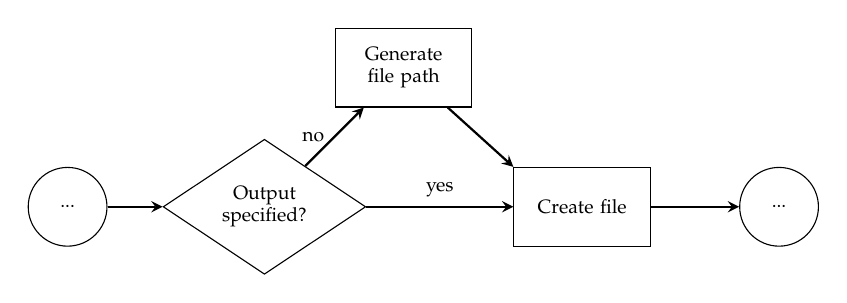
\begin{tikzpicture}[node distance=2.5cm,font=\scriptsize]
        \node (start) [startstop] {...};
        \node (pout) [decision, right of=start, text width=1.2cm, aspect=1.5] {Output specified?};
        
        \node (gen) [process, above right of=pout, text width=1.5cm] {Generate file path};
        \node (open) [process, below right of=gen, text width=1.5cm, xshift=0.5cm] {Create file};
        \node (stop) [startstop, right of=open] {...};
        
        \draw [arrow] (start) -- (pout);
        \draw [arrow] (pout) -- node[anchor=south] {yes} (open);
        \draw [arrow] (pout) -- node[anchor=east] {no} (gen);
        \draw [arrow] (gen) -- (open.north west);
        \draw [arrow] (open) -- (stop);
    \end{tikzpicture}
    \caption{A flow chart illustrating how the program branches differently based on the presence of a parameter.}
    \label{fig:ProgramBranching}
\end{figure}

Specifically for our program the user has the option to supply a name for the resulting output file. When this option is used the program can skip directly to creating the file rather than having to first generate a name based on the name of the input file. This example can be seen illustrated in figure \ref{fig:ProgramBranching}. In order to maximise program coverage for the analysis we want to avoid specifying a path for the output file since if specified the branch, where the file path is generated, would not be run.

This specific example is particularly relevant in this case since it happened to contain our programs' only memory leak. The memory leak was caused due to the pointer to the file path being stored in the same variable regardless of whether it was passed in as a program argument or dynamically allocated as part of the generation process. This made it impossible to determine if the path needed to be freed manually. To fix this we added an extra variable which we set before we generate the path string from the input file path. This variable is then used to check if the path needs to be freed once the program has finished.

\subsection{Manual testing}
One way to test functions and code while in the development phase is to do manual testing. It is very simple in the sense that it does not require any external tools. This means that it can be a lot more time consuming, because you have to make every test from the ground up, but that also means that it is very flexible, which is why we have done it so much. The goal of doing tests manually is to see if our functions behave as expected. This is done by giving the functions inputs that we think could give it problems, in many cases these are edge cases and special cases to make sure our program can handle even the more extreme scenarios.

One of the very simple manual tests we did was on the "tomorrow function". Given a date this function should return the next date. For this function the determined edge cases were when going from the end of a month to the beginning of a now month (inputting 31-01-2020 should return 01-02-2020), when going from the end of the year to the beginning of the new year (inputting 31-12-2020 should return 01-01-2021), and the special case was whether to include February 29th or not. The general behaviour of the function also had to be tested. To test all this we printed a Little more than a year in the terminal and checked that was as it was supposed to, in essence we had to see if we had printed a calendar in the terminal. The code can be seen on Listing \ref{lst:tomorrow_test}. A thing to note is that this test was made before the date struct had the week number as a member. 

\begin{lstlisting}[caption={tomorrow function testing.}, label={lst:tomorrow_test}, language=c]
/*tomorrow test*/
Date tomorrowTest = {1, 1, 2020};
for (int i = 0; i < 400; i++) {
    printf("D: %d, M: %d, Y: %d\n", 
           tomorrowTest.day,
           tomorrowTest.month,
           tomorrowTest.year);
    tomorrowTest = tomorrow(tomorrowTest);
}
\end{lstlisting}

With this test we got the behaviour we wanted and everything in the test went pretty well, except for leap years since that can change from year to year and the other things can not. That is not a major problem since the checking for leap years is a function itself which can also be tested. 

Manual testing can also be used to test more complex functions and that is what we did when we wanted to check the program output i.e the .csv file. Here it is pretty hard to see if everything is exactly how it should be, but it is very useful to find mistakes that need to be fixed. What ended up happening was that we would find something wrong with the schedule, fix it, and then find a new problem. We would iterate through this, slowly making the schedule better by fixing bugs, logic flows, and miscommunications. Some examples of what we had to fix these.

\begin{itemize}
    \item Weighting did not take work hours into account, which resulted in 24/7 working a couple of months, then having time off the rest of the year.
    \item When putting in the SH tag in a cell we did not show who had to work that day.
    \item Vacation days could get the RM tag, because the one who made the weighing function assumed that a vacation day would have zero hours of work time.
\end{itemize}

We had some more things that needed to be fixed before we could be happy with the final result of the schedule, but the process was basically the same. We also tried making some input that we would work as edge cases, one case where no one was working and one where everybody was working all the time. It was interesting to see how the program would act, but this was not what is was build for so the outcome did not help us all that much. Afterwards we found it hard to make some proper edge cases since the purpose of the program has always been to take a rough estimate of a schedule as an input. Therefore, it was hard to make an edge- or special case what also seemed realistic. 


\section{Solution comparison}
In this section we will look at the current solution at \siemens and our own solution to the problem, to see how they compare in different areas.

\subsection{Resulting schedule comparison}

Our system creates a work schedule that upholds all the union agreements, meaning that human mistakes are not possible as in the schedule currently made by \siemens. We have also made a grading system that would be unbiased regarding what days to add or remove, unless humans intervene through the criteria system. Our schedule however, does lack some of the visual attributes that the standard schedule has, when unedited. 

\begin{figure}[ht!]
    \centering
    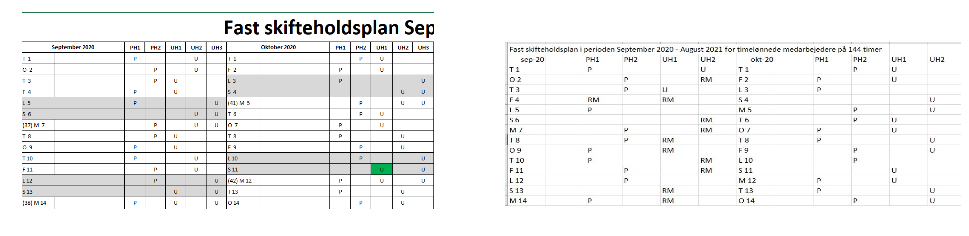
\includegraphics[width=\textwidth]{media/Comparison of Schedules.png}
    \caption{The left is the desired schedule, and the right is our unedited schedule}
    \label{fig:Our_Table}
\end{figure}

As shown above, the desired work schedule has color-coding, borderlines and a larger title. It is not possible through a .csv file to add colour and text-size to the schedule. That is why the person working with creating the schedule still needs to manually insert the different visual effects.

Our schedule also has a tendency to remove shifts earlier in the year, because it currently takes the first shift with highest priority, so the first SH-day would be removed, where a manual worker more likely would spread out the shifts removed. 

\subsection{Time comparison}
At last we want to show if our solution will actually be better than the system \siemens currently has. Our solution currently takes less than a second to read the input-file and write the output file. If we take into consideration that a user must also add the different visuals that the workers expect, that, in our own tests, took approximately 9 minutes, which was the time we used in testing. This means that the whole process of creating the work schedule can be done in less than 10 minutes.

Compared to the method that \siemens is currently using that takes about four uninterrupted hours, this method is much faster. It should also be noted that the person who is currently in charge of scheduling is very experienced in this area and would most likely be much faster than an inexperienced employee. Furthermore, this method does not mean you have to know the different requirements of making a schedule, the program does it for you. This means that the learning process of making a work schedule is also shortened to a few minutes.

So we can conclude that our solution is a viable improvement to the system currently used at \siemens, as it is both executed much faster and the time learned to master our system will be significantly lower, and much less prone to making mistakes, as it will create the work schedule reliably, and only need human input to make it look more appealing, and to specify different aspects if the work-schedule is not accepted.



% Conclusion
\chapter*{Conclusion}\addcontentsline{toc}{chapter}{Conclusion}
In this project our topic was scheduling, we decided to focus on \siemens since we had the opportunity to get some insider info and also some of the schedules. 

We started of by researching and writing a problem analysis. In the problem analysis there have been several different aspects that we have taken into account. These include \siemens' employee's needs and rights, existing solutions the union agreements as well as the more abstract term, fairness, among others. All of theses topics have been of great importance when building a solid foundation of knowledge which we could use to make a clear problem definition. With a tangible problem we could move on to the solution phase of the project.

In the second part of our report, which was focused on the development of the program we had to create. It was of utmost importance  to understand the requirements for the program as well as how the program flow should work. Because of the requirements we learned about in the problem analysis and our limited time scope, it was necessary to prioritize the features of our program. The list of priorities proved to be quite useful, since we always knew what to focus on.
It was also important to focus on the structure on the program itself both on an overall level between group members and on a more detailed level for what we had individually written. This helped organize and structure the development of the program.
Lastly, we documented the implementation of the program and the tests, which was quite important for helping the reader and ourselves get an overview of the finished program.

Finally, we can conclude that we have created a well functioning program, that takes the necessary requirements into account and is far more efficient than the current, manual scheduling method at \siemens. The program can easily be improved, but considering the time frame and what we managed to implement from our prioritized requirements list, we feel we have accomplished what we set out to do.

% Process Analysis
\chapter{Process Analysis}
Throughout this process analysis, we will in detail discuss the upsides and downsides to our project work and then reflect on that. This process analysis will then serve as a guideline for improvement for future projects.


\section{Initial problem} %initial problem
At the beginning of this project we were given a project-catalog, where we chose 'Vagtplanlægning' ('Work scheduling') as out subject. We had to delineate and define a problem. Luckily, a member of our group have a parent who works at \siemens, in a position with the function of creating the work schedule. She has to spend about a day on creating it, assuming it gets approved. If it does not, she will have to spend another whole day creating it from the bottom again. We chose this as a problem, since it is a real-life case, along with the possibility to get relevant people to actually user-test our solution, and compare it with what has been done previously.

We also made use of a Wh-diagram to narrow down our problem delineation. It has proven to quite a useful tool since it helped us understand the most important factors to take into account regarding our topic. In the end we were left with two possible problem delineations, focusing on improving the work scheduling to help the employer or doing it for the employee. As stated in our problem delineation, we chose to focus on the employee and making the schedule as fair as possible. There is no doubt the Wh-diagram has been particularly useful in that scenario, since it helped give us an overview of the interested parties as well as other important factors.

One of the most important factors we took into account when deciding on this topic, was that we wanted to work with a more authentic case instead of a purely theoretical one. That way we would also gain some practice when it came to working with real life problems, as we will be doing in future projects, for example our third semester project.

\section{From problem analysis to solution development}
The main purpose of the problem analysis was of course to get an understanding of \siemens's needs and understand the different interested parties as well as the definition of a fair schedule. The transition from working on the problem analysis to the solution development, since we had a solid foundation of knowledge upon which we could create our solution. It has therefore been quite easy to first and foremost outline the priorities of our program, since we only had about a month to create our program. 

One thing we did not do properly, regarding the use of our problem analysis in our solution development, was that we hardly used the analysis of existing solutions. Despite our research into already well functioning programs, we did not actually take these into consideration when developing our program. Another time we should probably go a bit more in depth of the analysis of different programs, look into their features and possible distinct advantages/disadvantages, and use that knowledge when creating our own program. However, the overall transition has been very smooth, and we have definitely experienced that the problem analysis has been very useful.
\begin{figure}[ht!]
    \centering
    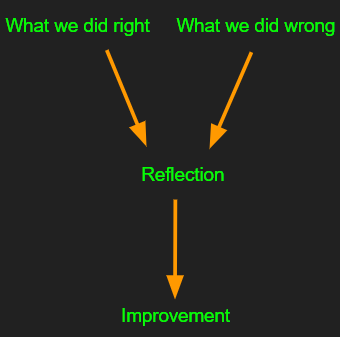
\includegraphics[width=5cm]{media/Gamma.PNG}
    \caption{The Gamma model: How we have worked in our process analysis}
    \label{fig:Gamma}
\end{figure}
\section{Status seminar}
Halfway through the P1-project we had a status seminar. We wanted to be sure our problem proposition was specified enough, and that the problem would be acceptable to solve. Although response from our opponent group was sparse, the feedback from our PBL teacher and supervisor was confirmation that we could continue with the problem proposition and actually begin designing and programming the solution to the scheduling problem of \siemens. There was of course also some suggestions for improvement of the report, which we implemented shortly after the status seminar.
\section{Project Management}
To manage our project, we have used several tools. The most prominent of these is Gitlab, since that has been used to keep track of both the development of the program and day to day planning, such as assigning tasks and planning meetings. Essentially, Gitlab has been an indispensable tool, since it has made it much easier for us to keep track of the project files and our progress.
Another useful tool has been Google Drive, since it has been useful for sharing notes, documents, and the data required for our project.


To manage our time and schedule the individual parts of our project, we have made a Gantt-chart in Google Sheets. It has been quite useful, since we always knew which part of the project we should work on. The Gannt-chart helped motivate us since there always was a deadline for each of the parts of our project, albeit an artificial one. Furthermore, it was quite useful when discussing the project with our supervisor, since we could always provide him a detailed plan of our future work on the project.

In conclusion, all the previously mentioned tools have been quite useful for their respective tasks and will most likely be used extensively in future projects.
\section{Group-teamwork}
Our teamwork has been nothing short of great since we all get along in our group. We are good at helping each other when need be, but we are also good at socializing and having fun on a daily basis in our group room. In our group contract, we have written that we must have one daily social activity of approximately 30 minutes, which is meant to strengthen our group bond. This daily activity can consist of anything from playing video games to discussing government funded artists. 
Our overall impression of this daily activity has been nothing but positive, since it has improved our group spirit.

However, the well functioning social dynamic of our group is also our groups Achilles' heel, since we sometimes spend too little time working on the project. One thing that we have done in an attempt to improve ourselves regarding our work morale, is setting daily goals. By doing that we have created a source of motivation for us. This has proven to be quite effective since our group has definitely increased its work morale and focus on the project compared to the days when we did not set any daily goals. 
\section{Working with our supervisor}
The work with our supervisor has been quite beneficial and useful to our group, since he has consistently provided our group with the necessary feedback, needed for our project. This has been done though both emails and weekly, virtual meetings on Microsoft Teams.

However, we had one incident where a misunderstanding occurred between our group and our supervisor. It was regarding some programming exercises that our supervisor expected us to complete, but our group wanted to focus on the problem analysis instead. These different expectations were somewhat quickly sorted out in one of our weekly meetings.
What we have learned from that incident was that communication is essential when working with your supervisor, since misunderstandings and different expectations regarding the project can easily occur. Therefore, it is of absolute importance to communicate often and effectively.

As previously mentioned, our group work has been mostly efficient and smooth. Therefore, we have also quite quickly worked through the top priorities of our programs, as mentioned in the "Specification and design" section. Our supervisor has been good at pressuring us to accomplish more than we originally set out to do. One of the topics that our supervisor asked us to investigate, was the time complexity of our scheduling algorithm. 
This has proven to be a difficult but rewarding task. In that sense it has been beneficial to us that we had a supervisor who could "pressure" us the right amount. That way we would get the most of our project work.

\section{What to improve in future projects}
In future projects we need to improve our usage of daily goals, as we need to make sure to make them every day, and also use them more effectively as guidelines to what we need to do. We would also like in future projects to be a bit more ambitious about our program and choice of topic, as this program, although a small one, still is very simple and did not need much advanced math or theory to solve. We also need to improve communication with our supervisor, as there has been a few miscommunications between the group and our supervisor. Furthermore, we need to make sure every member of the group knows what to work with, as there has been problems where members did not know what they should begin doing after completing their current task. This consequently meant that some group members did not work on anything while waiting to figure out what to do.

\section{Meta-reflection and conclusion}
So what can we do better in our next project? We need to make sure the first thing we do each day is to set some daily goals, and check if we reached the goal of yesterday. This way we are certain that what should be done today is clear, and it would also mean that everyone knew what to do the specific day. This would hopefully also make sure that everyone had something to work on, and therefore decrease or remove the non-productive time.

Our project work has overall been quite well functioning and effective, but there are a few areas, such as daily goals that we can still improve. It has definitely been interesting to work with a real life case, especially already in P1. It has forced us to take concepts like union agreements and fairness into consideration. We fully believe that this project has helped us learn not only about our very narrow problem delineation but about working with real cases as well.




\printbibliography[heading=bibintoc, title=References]
\label{bib:refs}

\appendix
\chapter{Local agreements \& data}\label{appendix:local-agreements}
The documents referred to by this appendix section are documents directly from \siemens. The documents should be available from the same source where you found or received this report. The local agreement consists of three PDF documents. The data is a set of multiple spreadsheets. In addition a \verb|.csv| version of the file that will given to the program as input is also included within this appendix.

% Overleaf files
% local agreements: sections/appendices/Siemens Gamesa local agreements 2020-2021/*
% example input file: sections/appendices/example-input-b.csv
\chapter{Full schedule pictures}\label{appendix:schedules}
In the figure that can be seen in section \ref{section:ap-b1} of this appendix is an image of the input schedule. In section \ref{section:ap-b2} an example of what the schedule look like after the program has been run.

\clearpage
\section{Input schedule}
\label{section:ap-b1}
\begin{figure}[hb!]
    \centering
    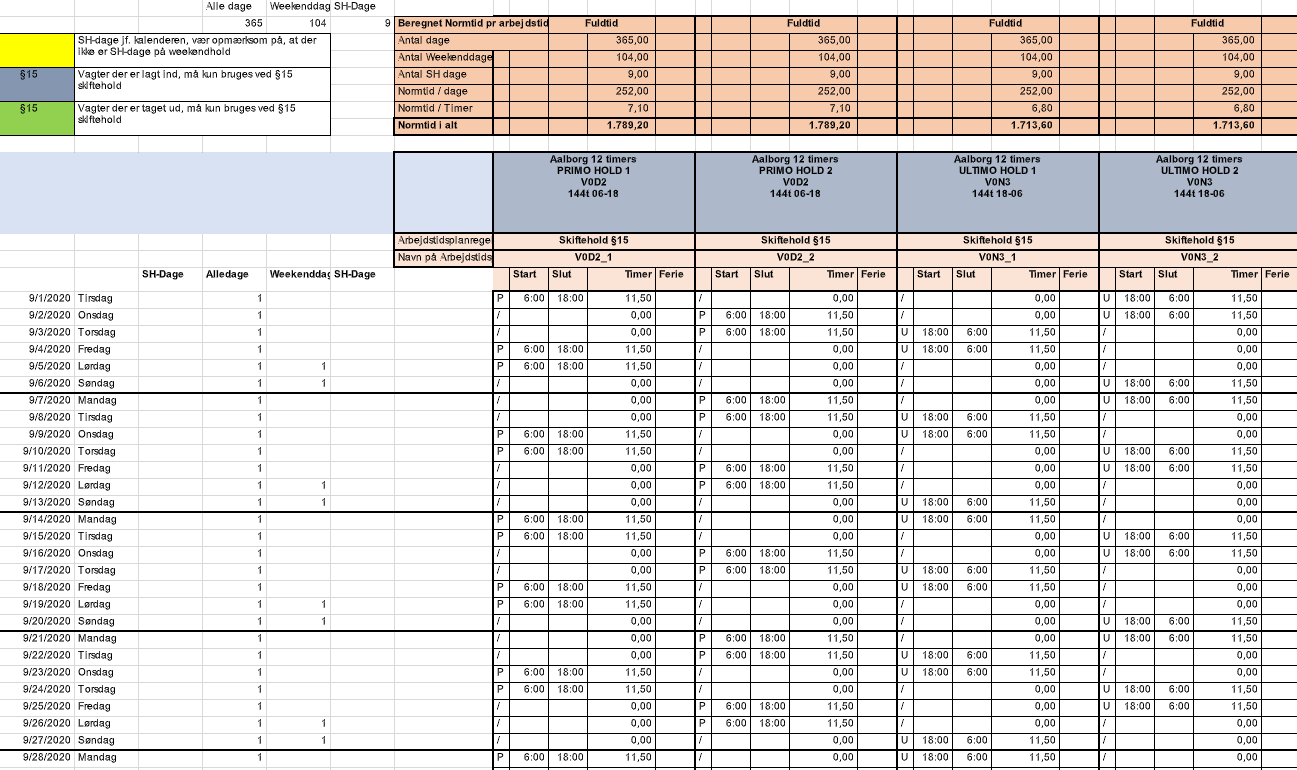
\includegraphics[angle=-90,origin=c,width=\textwidth-32pt]{sections/appendices/Schedules/Template.png}
    \label{fig:appendixTemplate}
\end{figure}

\clearpage
\section{Resulting schedule}
\label{section:ap-b2}
\begin{figure}[hb!]
    \centering
    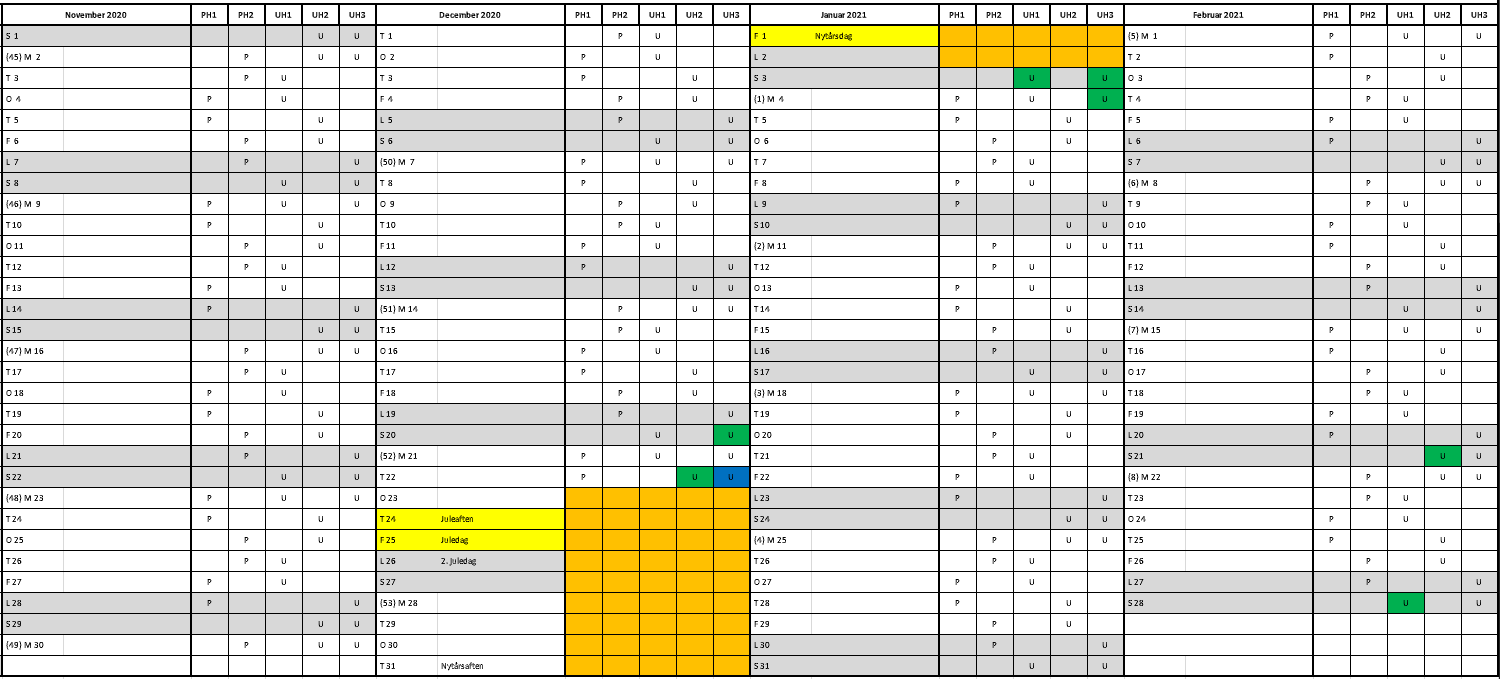
\includegraphics[angle=-90,origin=c,width=\textwidth-106pt]{sections/appendices/Schedules/Fixed.png}
    \label{fig:appendixFixed}
\end{figure}


\end{document}

